% Template for a Computer Science Tripos Part II project dissertation
\documentclass[12pt,a4paper,oneside]{report}
\usepackage{setspace}
\usepackage[pdfborder={0 0 0}]{hyperref}    % turns references into hyperlinks
\usepackage[margin=20mm]{geometry}  % adjusts page layout
\usepackage{graphicx}  % allows inclusion of PDF, PNG and JPG images
\usepackage{verbatim}
\usepackage{docmute}   % only needed to allow inclusion of proposal.tex
\usepackage{booktabs} %For professional formatting of tables
\usepackage[numbers]{natbib} %For formatting of references
\usepackage[toc,page]{appendix}
\usepackage{pdfpages} %For inserting PDF into latex source file
\usepackage{listings}

%User-introduced library and macros

\usepackage[T1]{fontenc}
\usepackage[utf8]{inputenc}
\usepackage{amsmath}
\usepackage{amsthm}
\usepackage{amssymb}
\usepackage{bbold}
\usepackage{tikz}
\usepackage{subcaption}
\usepackage{xcolor}
\usepackage{multirow}
\usepackage{booktabs}
\usepackage{makecell}
\usepackage{tabularx}
\usepackage{float}
\usepackage{booktabs} % For \toprule, \midrule, \bottomrule
\usepackage{ragged2e} % For better text alignment in narrow columns
\usepackage{caption}
\usepackage{placeins}
\usepackage{thmtools}
\usepackage{thm-restate}
\usepackage{titlesec}
\usepackage{enumitem}

% \includeonly{preparation/preparation, appendices/maths-defs-proofs, appendices/additional-code-listings}

\captionsetup{justification=centering, singlelinecheck=false}

\newfloat{algfloat}{htbp}{lop}
\floatname{algfloat}{Algorithm}
\def\lstfloatautorefname{Algorithm}

% Define a custom column type for left-aligned wrapping
\newcolumntype{L}{>{\RaggedRight\arraybackslash}X}

\usetikzlibrary{positioning, quotes, arrows.meta, calc, matrix, fit, backgrounds, decorations.pathreplacing}

\tikzset{
    deparrow/.style={
        -Stealth, 
        red, 
        line width=0.8pt, 
        % opacity=0.3, 
        shorten >=2pt, 
        shorten <=2pt
    },
    gdeparrow/.style={
        -Stealth, 
        gray, 
        line width=0.8pt, 
        % opacity=0.3, 
        shorten >=2pt, 
        shorten <=2pt,
        dashed
    }
}

\newcommand{\marker}[1]{\tikz[remember picture, overlay, baseline=(#1.base)] \node (#1) {};}
% \newcommand{\marker}[1]{\tikz[remember picture, overlay] \node[anchor=base, inner sep=0pt] (#1) {\strut};}
\newcommand{\offset}[1]{\protect\llap{\tiny\ttfamily\color{gray}#1\quad}}

\theoremstyle{definition}
\newtheorem{theorem}{Theorem}[section]
\newtheorem{definition}{Definition}[section]
\newtheorem{corollary}{Corollary}[section]

\hbadness=10000

\definecolor{codegray}{rgb}{0.5,0.5,0.5}

\lstdefinestyle{codestyle}{
    commentstyle=\color{codegray},
    numberstyle=\tiny,
    basicstyle=\ttfamily\footnotesize,
    breakatwhitespace=false,
    breaklines=true,
    captionpos=b,
    keepspaces=true,
    numbers=left,
    numbersep=5pt,
    showspaces=false,
    showstringspaces=false,
    showtabs=false,
    tabsize=2,
    frame=single
}

\lstset{style=codestyle}

% 1. Slash the massive top margin
% \titlespacing*{<command>}{<left>}{<before-sep>}{<after-sep>}
% Changing the <before-sep> to a negative value pulls the chapter title up.
\titlespacing*{\chapter}{0pt}{-20pt}{30pt}

% 2. Recreate the clean visual style from your example
\titleformat{\chapter}[display]
  {\normalfont\centering} % Centers the text and sets a base size
  {\MakeUppercase{\chaptertitlename}\ \thechapter} % "CHAPTER 3"
  {5pt} % Space between "CHAPTER 3" and the line
  {\Huge\bfseries} % Draws the line, adds space, formats title

%For a more accurate word count
%TC:envir table 0 1
%TC:envir table* 0 1
%TC:envir tabular [ignore] word
%TC:envir displaymath 0 word
%TC:envir math 0 word
%TC:envir listings 0 1
%TC:envir comment 0 0


%For inserting index
\usepackage{makeidx}
\makeindex
%\newcommand{\printthesisindex}{%
%    \cleardoublepage%
%    \phantomsection%
%    \addcontentsline{toc}{chapter}{Index}%
%    \printindex}

%Commands for entering line breaks
\usepackage{setspace}
% \onehalfspacing
\setlength{\parindent}{0pt}
\setlength{\parskip}{1.5ex plus0.5ex minus0.2ex}
% \renewcommand\baselinestretch{1.2}

\raggedbottom                           % try to avoid widows and orphans
\sloppy
\clubpenalty1000%
\widowpenalty1000%


\begin{document}

%Don't count text outside the main body within the word count
%tc:ignore

%%%%%%%%%%%%%%%%%%%%%%%%%%%%%%%%%%%%%%%%%%%%%%%%%%%%%%%%%%%%%%%%%%%%%%%%
% Title

\pagestyle{empty}

\rightline{\LARGE \textbf{3450C}}
%3450C

\vspace*{60mm}
\begin{center}
\Huge
\textbf{Efficient instruction-level parallelism analysis using tropical semiring `matrix multiplication'} \\[5mm]
Computer Science Tripos -- Part II \\[5mm]
\today  % today's date
\end{center}

%%%%%%%%%%%%%%%%%%%%%%%%%%%%%%%%%%%%%%%%%%%%%%%%%%%%%%%%%%%%%%%%%%%%%%%%%%%%%%%%
%%
%% Declaration
%%
%%%%%
 
\newpage
\section*{Declaration}

I, the candidate for Part II of the Computer Science Tripos with Blind Grading Number 3450C, hereby declare that this
report and the work described in it are my own work, unaided except as may be specified below, and that the report does
not contain material that has already been used to any substantial extent for a comparable purpose. In preparation of
this report, I adhered to the Department of Computer Science and Technology AI Policy.
I am content for my report to be made available to the students and staff of the University.

\medskip
\leftline{Date: \today.}

%%%%%%%%%%%%%%%%%%%%%%%%%%%%%%%%%%%%%%%%%%%%%%%%%%%%%%%%%%%%%%%%%%%%%%%%%%%%%%
% Proforma, table of contents and list of figures

%%%%%%%%%%%%%%%%%%%%%%%%%%%%%%%%%%%%%%%%%%%%%%%%%%%%%%%%%%%%%%%%%%%%%%%%%%%%%%%%
%%
%% Proforma
%%
%%%%%

\chapter*{Proforma}

\begingroup
\sloppy

\textbf{Candidate number}: 3450C \\
\textbf{Project title}: Efficient instruction-level parallelism analysis using tropical semiring `matrix multiplication' \\
\textbf{Examination}: Computer Science Tripos -- Part II, May 2026  \\
\textbf{Word count}: 11619 \footnotemark[1]\\
\textbf{Code line count}: 4534 \footnotemark[2]\\
\textbf{Project originator}: Alexandra Chadwick, \textit{awc32} \\
\textbf{Day-to-day supervisor}: Alexandra Chadwick, \textit{awc32}\\
\textbf{Marking supervisor}: Robert Mullins, \textit{rdm34}\\
%\textbf{(Whether approval from the Departmental Ethics Committee was requested, whether it was approved, and the Ethics Committee case number if applicable.)} \\


\footnotetext[1]{computed
using \texttt{textcount}
}
\stepcounter{footnote}
\footnotetext[2]{computed
using \texttt{cloc}
}

\endgroup

\section*{Original aims of the project}

Classical techniques for calculating the upper bound of instruction level parallelism in limit studies involve 
sequential algorithms that restrict efficiency.
This project explores a novel matrix-based technique for calculating the upper bound of instruction level parallelism
in a program. The objective was to show that this approach offers better performance than traditional analysis
techniques, at the cost of greater use of memory, by applying data-driven and parallel optimisations.

\section*{Work completed}

The project successfully met all core objectives and explored most extensions. The extension on through-memory dependencies 
stated in the proposal was ultimately not considered, and the work on GPU-based compute did not yield the expected 
performance benefits. I successfully built several iterations of a pipeline that computed the critical paths in program 
execution traces, and evaluated the effect of several optimisations and strategies, both data-driven and hardware-based.

\section*{Special difficulties}

None.

\listoffigures
\listoftables

%%%%%%%%%%%%%%%%%%%%%%%%%%%%%%%%%%%%%%%%%%%%%%%%%%%%%%%%%%%%%%%%%%%%%%%%%%%%%%%%
%%
%% Acknowledgements
%%
%%%%%

%%%%%%%%%%%%%%%%%%%%%%%%%%%%%%%%%%%%%%%%%%%%%%%%%%%%%%%%%%%%%%%%%%%%%%%%%%%%%%%%
%%
%% Table of contents
%%
%%%%%

\tableofcontents

\newpage

%%%%%%%%%%%%%%%%%%%%%%%%%%%%%%%%%%%%%%%%%%%%%%%%%%%%%%%%%%%%%%%%%%%%%%%
% now for the chapters

\pagestyle{headings}

%tc:endignore

\chapter{Introduction}

This project explores a novel matrix-based technique for calculating the upper bound of instruction level parallelism
in a program. This project shows that this approach offers better performance than traditional analysis techniques,
at the cost of greater use of memory.

\section{Background: ILP and limit studies} \label{intro:background}

\textit{Instruction level parallelism} (ILP) is the simultaneous execution of independent instructions in a computer processor~\cite{hennessy_patterson}.
A pair of instructions from a thread of execution are independent when there exist no dependencies (specifically data,
control or structural dependencies) between them. An instruction dependent on a previous one must be executed strictly
after the former has completed execution to ensure correct execution of the entire program.

Modern superscalar processors exploit ILP to increase throughput and hide latency \cite{shen2013modern}. The absolute limit of 
exploitable ILP is dependent on the structure of the executed program. A dynamic execution of a program will have a
`critical path' of instructions, each data-dependent on the previous, that have to be executed sequentially.

To understand these theoretical limits, studies are conducted to measure the maximum ILP available, through analysis 
on dynamic execution traces. Tools are used to build a \textit{dynamic dependency graph} (DDG), where nodes represent dynamically 
executed instructions, and edges represent the dependencies between them. The program's maximum available ILP is 
calculated by dividing the total number of executed instructions by the length of the longest path (the critical path)
through the DDG \cite{wall-ilp}. An example DDG is shown in Figure \ref{fig:DDG}.

\begin{figure}[ht]
    \rule{\textwidth}{0.5pt}\vspace{0.2cm}

    \centering
    % LEFT SIDE: Execution Trace
    \begin{minipage}[t]{0.35\textwidth}
        \centering
        \textit{Execution Trace} \\[1em]
        {\ttfamily\small
        \begin{tabular}{l}
        load r0, A \\
        load r1, B \\
        r4 $\leftarrow$ r0 + r1 \\
        load r2, C \\
        load r3, D \\
        r5 $\leftarrow$ r2 + r3 \\
        r6 $\leftarrow$ r4 + r5 \\
        store r6, S
        \end{tabular}}
    \end{minipage}
    \hfill
    % RIGHT SIDE: Dynamic Dependency Graph
    \begin{minipage}[t]{0.55\textwidth}
        \centering
        \textit{Dynamic Dependency Graph} \\[1em]
        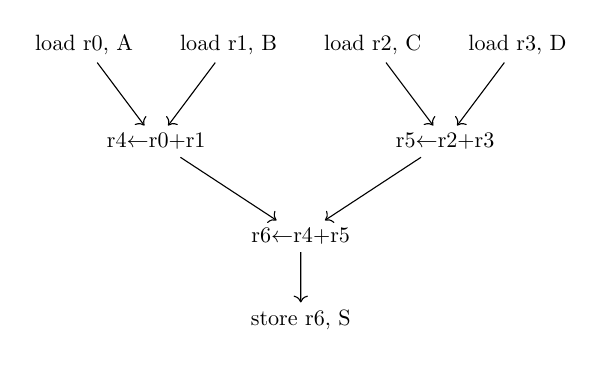
\begin{tikzpicture}[scale=0.8, every node/.style={transform shape}]
            \node (a0) {load r0, A};
            \node [right=0.5cm of a0] (a1) {load r1, B};
            \node [right=0.5cm of a1] (a2) {load r2, C};
            \node [right=0.5cm of a2] (a3) {load r3, D};

            \node (b0) [below=1cm of $(a0.south)!0.5!(a1.south)$] {r4$\leftarrow$r0+r1};
            \node (b1) [below=1cm of $(a2.south)!0.5!(a3.south)$] {r5$\leftarrow$r2+r3};

            \node (c0) [below=1cm of $(b0.south)!0.5!(b1.south)$] {r6$\leftarrow$r4+r5};
            \node (d0) [below=0.8cm of c0] {store r6, S};

            \draw[->] (a0) -- (b0);
            \draw[->] (a1) -- (b0);
            \draw[->] (a2) -- (b1);
            \draw[->] (a3) -- (b1);
            \draw[->] (b0) -- (c0);
            \draw[->] (b1) -- (c0);
            \draw[->] (c0) -- (d0);
        \end{tikzpicture}
    \end{minipage}

    \caption{Example dynamic dependency graph \cite{ddg}}
    \label{fig:DDG}
    \vspace{0.1cm}\rule{\textwidth}{0.5pt}
\end{figure}

\section{Motivation} \label{intro:motivation}

Traditionally, limit studies compute this longest path using a single-pass sequential sweep over the execution trace.~\cite{wall-ilp, ilp-spec95, perpi}
At each step they calculate the length of dependency paths ending at each register, and pick out the longest path at the 
end of the trace. Because the algorithm traverses the trace sequentially to propagate
dependencies, it cannot be heavily parallelised, nor can it exploit the memoisation of program stuctures such as loops.
This sequentiality limits the ability to handle realistic execution traces containing trillions of instructions,
which is important for capturing the effects of long-term dependencies found in complex, real-world 
software. Furthermore, this analysis is rarely a single-pass operation. Limit studies evaluate programs across comprehensive 
benchmark suites under various parameters, such as restricted instruction windows or different branch prediction models~\cite{wall-ilp, future-ilp, ilp-spec95}.

To break this sequential bottleneck, Chadwick \cite{Chadderz} proposes a matrix-based approach. By representing instruction 
dependencies as matrices, and using matrix multiplication in the max-tropical semiring, computing the longest path in
the DDG becomes a problem of reducing a large expression of matrix multiplications.
Because matrix multiplication is associative, the expression can be evaluated in any order, and intermediate results 
fully encode the dependency information of the instructions they range over. This enables a range of optimisations when 
computing ILP limits, including thread-parallelisation of computations and memoisation of repetitive intermediate results.
One additional benefit of the associativity of the matrix expression is that it trivialises instruction window scaling.
Consider three windows of instructions: A, B, and C (which is comprised of windows A and B consecutively).

% \begin{center}
% 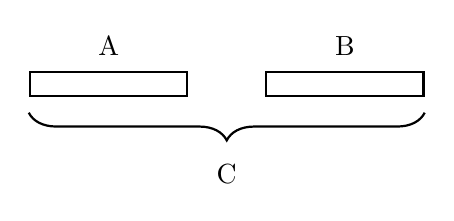
\begin{tikzpicture}

    % Define the two rectangles
    \node[draw, rectangle, minimum width=2cm, minimum height=0.3cm, thick] (boxA) at (0,0) {};
    \node[draw, rectangle, minimum width=2cm, minimum height=0.3cm, thick] (boxB) at (3,0) {};

    % Add labels A and B above the rectangles
    \node at (boxA.north) [above=2pt] {A};
    \node at (boxB.north) [above=2pt] {B};

    % Draw the brace spanning from the bottom-left of A to the bottom-right of B
    % 'mirror' puts the brace below the line
    \draw [decorate, decoration={brace, amplitude=10pt, mirror}, thick] 
        ([yshift=-0.2cm]boxA.south west) -- ([yshift=-0.2cm]boxB.south east) 
        node[midway, below=15pt] {C};

\end{tikzpicture}

% \end{center}

To compute ILP information for each window, the traditional approach must be executed 3 times, once for 
each window. However, the matrix-based approach will only need to run twice, on A and B, and the dependency 
information matrix for C can simply be obtained by multiplying the result matrices from A and B.

\section{Contributions}

In this project, I explore several approaches for offline computation of the upper limit of ILP in a program, and
compare their performance.
The first is a sequential approach mirroring the classical trace-analysis techniques, based on the PerPI tool \cite{perpi}. We will 
refer to this as the `naive baseline' throughout the project.
I then explore Chadwick's matrix-based approach, implementing a series of algorithmic and hardware-level optimisations.
Specifically, I use sparse matrix representations to reduce memory overhead, and develop data-level heuristics to 
determine optimal expression evaluation orders. Finally, I introduce parallel optimisations, leveraging multi-threading 
and accelerator-level parallelism to distribute the computational workload.

I show experimentally in Section \ref{eval:holistic-pipeline}
that a single-threaded pipeline equipped with the data-driven optimisations matches or beats the performance 
of the naive baseline. Furthermore, by distributing expression reduction and matrix multiplication workloads over 
multiple cores, I show that the parallel approach is at least twice as fast as the baseline,
demonstrating the scalability of the matrix-based approach in analysing large execution traces.


\chapter{Preparation}

\section{Understanding the matrix-based approach}

{\footnotesize\itshape
The applications of tropical semirings to dynamic dependency graphs, particularly the sections on
register-only longest chains (\ref{prep:register-only-chains})
and alternative graph structures (\ref{prep:alternative-matrix-struct})
are closely adapted from the methodologies established by Chadwick \cite{Chadderz}.}

\subsection{The tropical semiring (max-plus algebra)}

Tropical analysis is a branch of pure mathematics that is the study of the tropical semiring.
There are two variants of the tropical semiring, namely the min-plus and max-plus algebras.
We will use the max-plus convention to apply to \textit{longest} paths in directed acyclic graphs.

 
% Define tropical semiring and operations 

\begin{definition}[Semiring] \label{def:semiring}
  A semiring \cite{Wandsnider2020} is a set $R$ along with two operations, addition (+) and multiplication ($\cdot$), which satisfy the 
  following axioms:

  \begin{enumerate}
    \item Addition is associative and commutative.
    \item Multiplication is associative.
    \item There exists an additive identity, which we usually call $\mathbb{0}$. Additionally, $\mathbb{0}$ annihilates 
      $R$, that is, for all $x \in R$, $\mathbb{0} \cdot x = x \cdot \mathbb{0} = \mathbb{0}$.
    \item There exists a multiplicative identity, which we usually call $\mathbb{1}$.
    \item Multiplication left and right distributes over addition.
  \end{enumerate}
\end{definition}

\begin{definition}[Tropical semiring]
  The tropical semiring \cite{Wandsnider2020}, or max-plus algebra, is the object $(\mathbb{R} \cup \{-\infty\}, \oplus, \odot)$ with operations 
defined as:

$$
\begin{aligned}
  a\oplus b &= \max(a,b) \\
  a\odot b &= a+b
\end{aligned}
$$

\end{definition}

The tropical semiring satisfies the axioms of a semiring from Definition \ref{def:semiring}. It
is not a ring as the max operator does not have an inverse.

% Define matrix multiplication in the context of the tropical semiring

\begin{definition}[Matrix operations in the tropical semiring]
For any $n\times n$ matrices $X = (x_{ij})$ and $Y = (y_{ij})$, the entries of $U = X \oplus Y$ and $V = X \odot Y$
are calculated as \cite{krivulin2012maxplusalgebraapproachmodelling}

$$
u_{ij} = x_{ij} \oplus y_{ij}, \text{ and } v_{ij} = \displaystyle\sum_{k=1}^{n} \! {}_{\oplus} x_{ik} \odot y_{kj}
$$

\end{definition}

The matrix operations $\oplus$ and $\odot$ are associative owing to the commutativity and associativity of the underlying 
addition operator, and that the multiplication operator distributes over addition.

\subsection{Longest paths in Directed Acyclic Graphs}


% Show how this applies to the longest-path problem

As established previously, finding the length of the critical path in a program results in finding the longest path
in its DDG. It is noted that the max-plus version of the tropical semiring is applicable to finding the longest path
in a graph \cite{krivulin2012maxplusalgebraapproachmodelling}.

One algorithm \cite{Chadderz} to find the longest path between nodes $A$ and $B$ in a graph is to recursively take the 
maximum of all path lengths from all neighbours of $A$ to $B$, plus the cost of the edge from $A$ to the chosen
neighbour. We can see that this amounts to a Bellman recursion equation \cite{Bellman:DynamicProgramming}
involving only the max and plus operators: 

$$
v(A,B) = 
\begin{cases}
0 &\text{ if } A = B \\
\max_{\forall C . A \to C} \{\mathrm{weight}(A \to C) + v(C,B))\}, &\text{ otherwise } \\
\end{cases}
$$

We can observe that, if we have an adjacency matrix (where the cells in that matrix represent the cost of the edge
between the pair of nodes in that row/column, and $-\infty$ if there is no edge), performing tropical semiring 
matrix multiplication of this matrix with itself corresponds to one step of our longest-path algorithm.

Formally we consider an adjacency matrix $X^{2} = X \odot X$, and denote its entries by $x_{ij}^{(2)}$. We have that $x_{ij}^{(2)} = p$
if and only if there exists at least one path of length $p$ from node $i$ to node $j$ in the corresponding graph,
consisting of at most two edges, and that path is the longest such path. This extends to any integer exponent $q$
\cite{krivulin2012maxplusalgebraapproachmodelling}.

\begin{theorem}[Matrix exponentiation results in longest paths] \label{thm:mat-exp-longest-paths}

For any integer $q>0$, the matrix
$X^{q}$ has the entry $x_{ij}^{(q)} = p$ only if there is a path of length $p$ with at most $q$ edges from $i$ to $j$,
and that path is the longest such path.

\begin{proof}
  We proceed by induction on $q$, the maximum number of edges in the path.

  \textbf{Base case ($q = 1$):} Consider the matrix $X^1=X$. By the definition of an adjacency matrix, the entry  
  $x_{ij}^{(1)}$ is exactly the weight of the direct edge from node $i$ to node $j$. If no such edge exists, then 
  $x_{ij}^{(1)} = -\infty$. Thus, the base case holds: the entries represent their longest paths consisting of at most 
  one edge.

  \textbf{Inductive step:} Assume the claim holds for $q$. That is the matrix $X^{q}$ has entries $x_{ij}^{q}$ 
  representing the longest path from $i$ to $j$ using at most $q$ edges.
  We show that the claim holds for $q+1$. By definition, $X^{q+1} = X^{q} \odot X$
  The entry $x_{ij}^{(q+1)}$ is calculated as:
  $$x_{ij}^{(q+1)} = \sum_{k=1}^{n} \! {}_{\oplus} (x_{ik}^{(q)}\odot x_{kj})$$
  Translating this to the original operators:
  $$
  x_{ij}^{(q+1)} = \max_{1 \leq k \leq n} (x_{ik}^{(q)} + x_{kj})
  $$
  This lines up perfectly with the dynamic programming approach to finding the longest path. To find a longest path from
  node $i$ to node $j$, it checks every intermediate node $k$. It takes the longest known path from $i$ to $k$ of at most 
  $q$ edges (by the inductive hypothesis), and adds the direct edge cost from $k$ to $j$. By taking the maximum over all 
  intermediate nodes $k$, we find the absolute longest path from $i$ to $j$ of at most $q+1$ edges. Thus the claim holds 
  for all integers $q>0$.
\end{proof}

So, an adjacency matrix raised to the power infinity will converge to the longest distance matrix for that whole graph.
  
\end{theorem}


For example, consider the graph:
\begin{center}
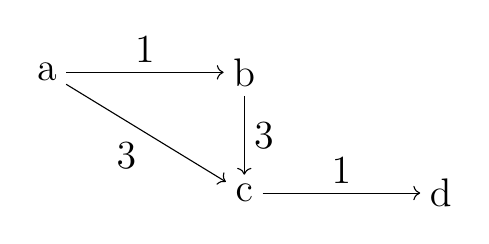
\begin{tikzpicture}[
    node distance=1cm and 2cm, % vertical and horizontal spacing
    every node/.style={font=\Large} % makes letters look like your image
]
    % Place the nodes
    \node (a) {a};
    \node (b) [right=of a] {b};
    \node (c) [below=of b] {c};
    \node (d) [right=of c] {d};

    % Draw the edges (undirected lines) with labels
    \draw [->] (a) -- node[above] {1} (b);
    \draw [->] (a) -- node[below left] {3} (c);
    \draw [->] (b) -- node[right] {3} (c);
    \draw [->] (c) -- node[above] {1} (d);
\end{tikzpicture}
\end{center}

The corresponding adjacency matrix would be:
$$
X = 
\begin{pmatrix}
  0 & 1 & 3 & -\infty \\ 
  -\infty & 0 & 3 & -\infty \\ 
  -\infty & -\infty & 0 & 1 \\
  -\infty & -\infty & -\infty & 0 \\
\end{pmatrix}
$$

So, in the tropical semiring:

$$
\begin{aligned}
  X^{2} &= 
  \begin{pmatrix}
    0 & 1 & 4 & 4 \\ 
    -\infty & 0 & 3 & 4 \\ 
    -\infty & -\infty & 0 & 1 \\ 
    -\infty & -\infty & -\infty & 0 \\
  \end{pmatrix} \\ 
  X^{3} &= 
  \begin{pmatrix}
    0 & 1 & 4 & 5 \\ 
    -\infty & 0 & 3 & 4 \\ 
    -\infty & -\infty & 0 & 1 \\ 
    -\infty & -\infty & -\infty & 0 \\
  \end{pmatrix} \\ 
        & = X^{4} = X^{5} = \dots = X^{\infty}
\end{aligned}
$$

This corresponds to the longest distance matrix between all pairs of nodes.

\subsection{Forming the DDG and register-only longest chains} \label{prep:register-only-chains}

As defined in Section \ref{intro:methodology}, a standard DDG represents 
each dynamically executed instruction as a single node. While this formulation is intuitive for visualising the program 
flow, the structure of the graph is arbitrary, and we would wish to impose a more rigid structure to allow for future
optimisations, as outlined in Section \ref{prep:alternative-matrix-struct}.
To do this, we can encode the transformation of the machine's dependency state from one cycle to the next.
We introduce a new expanded graph structure, which has one node per register per dynamic instruction.

Let us first consider the dependencies for instructions only affecting registers.
Since each instruction has a fixed set of registers which it accesses, it has a fixed dependency structure, and so each 
instruction in the program trace will have a fixed subgraph in the expanded DDG encoding its dependency information.

For example, we could encode the dependencies for the instruction \verb|R0 = ADD R1, R2| as the subgraph:

\begin{center}
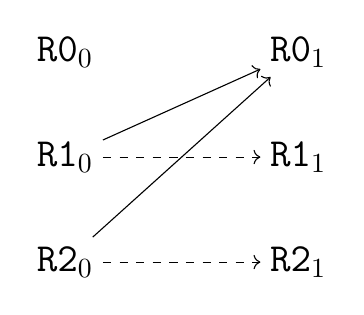
\begin{tikzpicture}[
    node distance=0.7cm and 2cm, % vertical and horizontal spacing
    every node/.style={font=\Large} % makes letters look like your image
]
    % Place the nodes
    \node (r0_0) {\verb|R0|$_{0}$};
    \node (r1_0) [below=of r0_0] {\verb|R1|$_{0}$};
    \node (r2_0) [below=of r1_0] {\verb|R2|$_{0}$};
    \node (r0_1) [right=of r0_0] {\verb|R0|$_{1}$};
    \node (r1_1) [below=of r0_1] {\verb|R1|$_{1}$};
    \node (r2_1) [below=of r1_1] {\verb|R2|$_{1}$};

    % Draw the edges
    \draw [->] (r1_0) -- (r0_1);
    \draw [->] (r2_0) -- (r0_1);

    % draw the zero-cost edges
    \draw [->, dashed] (r1_0) -- (r1_1);
    \draw [->, dashed] (r2_0) -- (r2_1);
\end{tikzpicture}

{\tiny dashed edges are 0 cost}
\end{center}

The instruction reads from \verb|R1| and \verb|R2| and uses these values to produce a new value stored in \verb|R0|.
On the left of the subgraph is the register state before the instruction execution; on the right is after. The 
characteristics of the subgraph are as follows:
\begin{itemize}
  \item Since the value \verb|R0|$_1$ is dependent on \verb|R1|$_0$ and \verb|R2|$_0$, there are cost-1 edges in the graph 
    from \verb|R1|$_0$ and \verb|R2|$_0$ to \verb|R0|$_1$, extending the dependency chain from the source registers to the 
    destination by 1 cycle.

  \item The values in \verb|R1| and \verb|R2| are unchanged by the instruction, so their respective states have 0-cost 
    edges between them. This allows dependency chains from the source registers to `skip over' this particular instruction 
    that does not affect them.

  \item Finally, since the value in \verb|R0| is modified, there is no 0-cost edge between the respective states, as the 
    old value is discarded and a new chain starts at the new value.
\end{itemize}


The full DDG will consist of several of these subgraphs, horizontally glued together, with one new set of dependency edges 
for each additional instruction.

The true critical path often involves memory operations, as a value may be copied to memory from a register, then 
potentially millions of instructions later that value is read into a register and used, contributing to a data dependency,
yet we have not accounted for this here. While Chadwick \cite{Chadderz} has suggested approaches to track through-memory
dependencies, this project will not do so, as they require dealing with much larger matrices or significantly complicating 
the structure of the datasets, which fell outside of the project's scope.

Unfortunately, even modest, realistic programs can have trillions of instructions in their 
traces, and so an adjacency matrix for the entire graph becomes unfeasible. However, we can use an alternative 
representation.

\subsection{Alternative graph representation} \label{prep:alternative-matrix-struct}

% Show how we arrange the DDG such that we can have a matrix representing dependencies of an instr.

We can see a particular structure in the DDGs we construct - they are more long than wide. While a 
standard $N \times N$ adjacency matrix (where $N$ is the total number of dynamically executed instructions) could 
map the graph, it is inefficient.
This is because, in the DDG, edges \textit{only} exist between adjacent columns.
Therefore, the full adjacency matrix $X$ is mostly filled with $-\infty$.
Instead, the DDG can be modelled as a sequence of adjacent columns. 
Consider an arbitrary graph with the property of being more long than wide:

\begin{center}
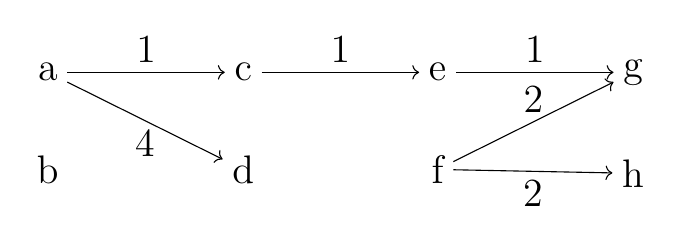
\begin{tikzpicture}[
    node distance=0.7cm and 2cm, % vertical and horizontal spacing
    every node/.style={font=\Large} % makes letters look like your image
]
    % Place the nodes
    \node (a) {a};
    \node (b) [below=of a] {b};
    \node (c) [right=of a] {c};
    \node (d) [below=of c] {d};
    \node (e) [right=of c] {e};
    \node (g) [right=of e] {g};
    \node (f) [below=of e] {f};
    \node (h) [below=of g] {h};

    % Draw the edges (undirected lines) with labels
    \draw [->] (a) -- node[above] {1} (c);
    \draw [->] (a) -- node[below] {4} (d);
    \draw [->] (c) -- node[above] {1} (e);
    \draw [->] (e) -- node[above] {1} (g);
    \draw [->] (f) -- node[above] {2} (g);
    \draw [->] (f) -- node[below] {2} (h);
\end{tikzpicture}
\end{center}

First of all, we modify the graph such that the longest path will always connected to the 
rightmost part of the graph, by adding extra nodes and cost-0 edges, and so also each path is connected to the first 
column similarly.

To utilize column-wise matrices for longest-path calculations, the graph must first be padded. We introduce a set of 
`dummy' nodes to the first and last columns, connected by 0-cost edges. This guarantees that any local path within the 
interior of the graph is extended to touch both the initial and final columns.

\begin{center}
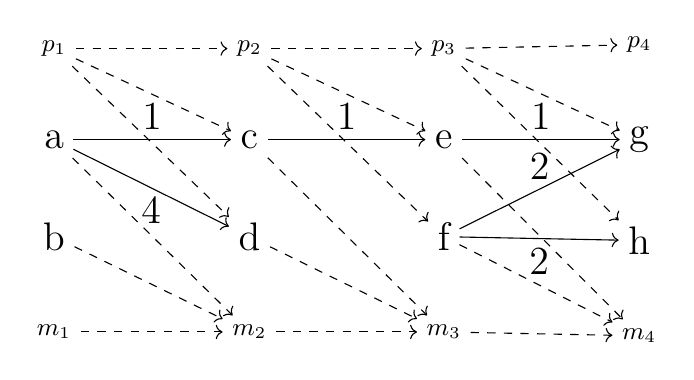
\begin{tikzpicture}[
    node distance=0.7cm and 2cm, % vertical and horizontal spacing
    every node/.style={font=\Large} % makes letters look like your image
]
    % Place the nodes
    \node (a) {a};
    \node (b) [below=of a] {b};
    \node (c) [right=of a] {c};
    \node (d) [below=of c] {d};
    \node (e) [right=of c] {e};
    \node (g) [right=of e] {g};
    \node (f) [below=of e] {f};
    \node (h) [below=of g] {h};

    \node (p1) [above=of a, font=\small] {$p_1$};
    \node (p2) [above=of c, font=\small] {$p_2$};
    \node (p3) [above=of e, font=\small] {$p_3$};
    \node (p4) [above=of g, font=\small] {$p_4$};

    \node (m1) [below=of b, font=\small] {$m_1$};
    \node (m2) [below=of d, font=\small] {$m_2$};
    \node (m3) [below=of f, font=\small] {$m_3$};
    \node (m4) [below=of h, font=\small] {$m_4$};

    % Draw the edges with labels
    \draw [->] (a) -- node[above] {1} (c);
    \draw [->] (a) -- node[below] {4} (d);
    \draw [->] (c) -- node[above] {1} (e);
    \draw [->] (e) -- node[above] {1} (g);
    \draw [->] (f) -- node[above] {2} (g);
    \draw [->] (f) -- node[below] {2} (h);

    % draw the zero-cost edges
    \draw [->, dashed] (p1) -- (p2);
    \draw [->, dashed] (p1) -- (c);
    \draw [->, dashed] (p1) -- (d);

    \draw [->, dashed] (p2) -- (p3);
    \draw [->, dashed] (p2) -- (e);
    \draw [->, dashed] (p2) -- (f);

    \draw [->, dashed] (p3) -- (p4);
    \draw [->, dashed] (p3) -- (g);
    \draw [->, dashed] (p3) -- (h);

    \draw [->, dashed] (a) -- (m2);
    \draw [->, dashed] (b) -- (m2);
    \draw [->, dashed] (m1) -- (m2);

    \draw [->, dashed] (c) -- (m3);
    \draw [->, dashed] (d) -- (m3);
    \draw [->, dashed] (m2) -- (m3);

    \draw [->, dashed] (e) -- (m4);
    \draw [->, dashed] (f) -- (m4);
    \draw [->, dashed] (m3) -- (m4);
\end{tikzpicture}

{\tiny dashed edges are 0 cost}
\end{center}

Now we can represent the graph with one matrix per adjacent-column pair, encoding the connectivity between those two
columns. The connectivity between the first two columns is represented as:

\[
  X_{1,2} = 
  \begin{pmatrix}
  0 & 0 & 0 & -\infty \\
  -\infty & 1 & 4 & 0 \\
  -\infty & -\infty & -\infty & 0 \\
  -\infty & -\infty & -\infty & 0 
  \end{pmatrix}
\]

where the $m$th row and $n$th column of this matrix represent the connection from the $m$th node in the first column of 
the graph to the $n$th node in the second column of the graph.

The remaining two column pairs are represented as:

\[
  \begin{aligned}
    X_{2,3} &= 
    \begin{pmatrix}
    0 & 0 & 0 & -\infty \\
    -\infty & 1 & -\infty & 0 \\
    -\infty & -\infty & -\infty & 0 \\
    -\infty & -\infty & -\infty & 0 
    \end{pmatrix} \\
    X_{3,4} &= 
    \begin{pmatrix}
    0 & 0 & 0 & -\infty \\
    -\infty & 1 & -\infty & 0 \\
    -\infty & 2 & 2 & 0 \\
    -\infty & -\infty & -\infty & 0 
    \end{pmatrix}\\
  \end{aligned}
\]

These matrices are each $4 \times 4$ whereas a full adjacency matrix for the original graph would be $7 \times 7$.
We can see that the column-wise matrices will use less storage than the adjacency matrix (48 integers vs 49 integers),
and this alternative becomes increasingly favourable as the graph gets longer.


In the tropical semiring, computing the matrix product

\[
  X_{3,4} \odot X_{2,3} \odot X_{1,2} = \begin{pmatrix}
  0 & 2 & 2 & 1 \\
  -\infty & 3 & -\infty & 4 \\
  -\infty & -\infty & -\infty & 0 \\
  -\infty & -\infty & -\infty & 0 
\end{pmatrix}
\]
yields a matrix representing the longest path from the $m$th node in the first column the $n$th node in the final 
column of the graph. Because we have ensured every path in the graph connects to the first and last column, the largest 
individual value in this matrix is the length of the longest path in the graph, namely the path of length 4 connecting 
from $a$ in the first column, to $m_4$ in the final column, via $d$ and $m_3$.

The correctness of the column-wise approach for calculating longest paths in graphs is a corollary that follows directly 
from Theorem \ref{thm:mat-exp-longest-paths}.

\begin{corollary}[Correctness of the column-wise formulation]
  In a standard adjacency matrix $X$, computing $X^{q}$ checks every possible intermediate node 
  $k$ in the entire graph to find paths of length $q$, as shown by Theorem \ref{thm:mat-exp-longest-paths}.

  In a column-wise representation of the DDG, when we multiply adjacent column matrices (e.g., $X_{2,3} \odot X_{1,2}$),
  we are simply performing the exact operations for finding the longest path between columns 1 and 3,
  but restricted only to the intermediate nodes $k$ located in column $2$.
  This is valid as edges in the DDG only exist between adjacent columns.

  Because the padding of 0 cost edges ensures every path spans from the first column to the final column, multiplying 
  all consecutive column matrices sequentially computes the maximum path length across the entire graph.
\end{corollary}

This defines the final shape of the data that we will be working on as a mathematical expression consisting of a
series of matrix multiplications. 

We can use the column-wise approach to represent the alternative DDG structure from Section \ref{prep:register-only-chains}.
Because each dynamic instruction has a static set of dependencies, represented by a matrix, and because there are many 
more dynamic instructions in the DDG than the number of static instructions in the program, we will see frequent reuse 
of matrices in the equation, allowing us to find and exploit common patterns, and further reducing the actual memory 
required to store the DDG.

\section{Datasets}

I decided to use execution traces of various coreutils programs as input when testing and benchmarking the analysis tool.
These programs are familiar to developers and display a range of properties that are favourable to several optimisations 
we explore.

\subsection{Dataset listing}

The chosen program executions are:

\begin{itemize}
  \item \verb|cksum < urandom_1MiB.bin|

  the {\color{blue}\textbf{\href{https://www.gnu.org/software/coreutils/manual/html\_node/cksum-invocation.html}{coreutils cksum utility}}} ,
  v8.32 running on AArch64, calculating the CRC of a 1MiB file of random bytes.

  \item \verb|cksum < urandom_32MiB.bin|

  the {\color{blue}\textbf{\href{https://www.gnu.org/software/coreutils/manual/html\_node/cksum-invocation.html}{coreutils cksum utility}}} ,
  v8.32 running on AArch64, calculating the CRC of a 32MiB file of random bytes.

  \item \verb|factor 9696593808888933181586|

  the {\color{blue}\textbf{\href{https://www.gnu.org/software/coreutils/manual/html\_node/factor-invocation.html}{coreutils factor utility}}} ,
  v8.32 running on AArch64, 9696593808888933181586.

  \item \verb|sha1sum < urandom_1MiB.bin|

  the {\color{blue}\textbf{\href{https://www.gnu.org/software/coreutils/manual/html\_node/sha1sum-invocation.html}{coreutils sha1sum utility}}} ,
  v8.32 running on AArch64, computing the SHA1 message digest of a 1MiB file of random bytes.

  \item \verb|sort < urandom_2000_lines.txt|

  the {\color{blue}\textbf{\href{https://www.gnu.org/software/coreutils/manual/html\_node/sort-invocation.html}{coreutils sort utility}}} ,
  v8.32 running on AArch64, sorting a 2000 line text file of hexadecimal digits encoding random bytes.

  \item \verb|shuf --random-source=urandom_1MiB.bin urandom_34953_lines.txt|

  the {\color{blue}\textbf{\href{https://www.gnu.org/software/coreutils/manual/html\_node/shuf-invocation.html}{coreutils shuf utility}}} ,
  v8.32 running on AArch64, shuffling a 34953 line text file of hexadecimal digits encoding random bytes.
\end{itemize}

The source data can be found at \url{https://www.cl.cam.ac.uk/~awc32/cam-only/tropical-ilp-p2p/}. The traces were 
collected by Alexandra Chadwick (\textit{awc32}) using custom tooling.

\subsection{Data properties}

\begin{table}[ht]
\begin{center}
\begin{tabular}{lcccccc}
  \toprule
  \textbf{Dataset} & \textbf{Instructions} & \textbf{Basic Blocks} & \multicolumn{4}{c}{\textbf{Biggest Pattern}\protect\footnotemark} \\
  \cmidrule(l){4-7}
  & (Total) & (Total) & Period\protect\footnotemark & ACI\protect\footnotemark & TI\protect\footnotemark & Coverage\\
  \midrule
  cksum   & 7526926   & 1068940  & 1 & 65535 & 1048560 & 98.1\% \\
  cksum32 & -         & -        & - & - & - & - \\
  factor  & 220632540 & 18074022 & 5 & 20 & 993556 & 27.5\% \\
  sha1sum & 16994993  & 91070    & 1 & 3 & 49155 & 54.0\% \\
  sort    & 10943690  & 1216990  & 17 & 2 & 7536 & 10.5\% \\
  shuf    & 16361747  & 2147424  & 30 & 3 & 16007 & 22.3\% \\
  \bottomrule
\end{tabular}
\end{center}
\caption{Summary of trace analysis on the selected data.}
\label{tbl:trace-analysis}
\end{table}

\footnotetext[1]{Results acquired with an analysis tool based on the loop simplifier in Section IMPLEMENTATION, using a 
window size of 5000 and a history size of 200. The `biggest' pattern in the program is that which covers the largest number 
of basic blocks}
\footnotetext[2]{Period is measured in length of basic blocks and is the length of one iteration of a pattern.}
\footnotetext[3]{Average Consecutive Iterations: The mean number of times a period of a pattern will repeat without interruption.}
\footnotetext[4]{Total Iterations: The total number of times a period of a pattern exists in the program trace.}

As shown in Table \ref{tbl:trace-analysis}, all datasets exhibit a `largest pattern' covering a significant proportion of the trace.
The datasets additionally have other similarly significant patterns not shown in the table.
These patterns can be exploited in two ways:

\begin{enumerate}
  \item Consecutive repetitions of matrices can be quickly reduced down into a single matrix using a quick exponentiation algorithm.
  \item The matrices making up one iteration of the loop can be multiplied together to obtain a singular matrix representing 
    the dependency information for that single iteration. All other iterations of that loop body can then be replaced with 
    the singular result matrix without any extra computation.
\end{enumerate}

\section{Project design}

This section outlines the software engineering methodology adopted during implementation, specification of the 
project requirements, and technical justification for the chosen tools.

\subsection{Software engineering}

For the project, I adopted the iterative spiral methodology. Given the experimental nature of performance optimisation, 
this methodology allowed for a repetitive cycle of planning, followed by implementation, and concluding with an 
evaluation phase where performance bottlenecks were identified to inform the next cycle.

To maintain codebase integrity during high-frequency iterations, code was regularly committed and pushed to GitHub,
using feature branches to implement large changes. Commits from branches were squashed upon merge to provide a clean, 
linear history of major architectural milestones.

\subsection{Project requirements}

% Use a must-should-could pattern for several sections
% MoSCoW

Requirements are listed in Table \ref{tbl:requirements-analysis}
and categorised by their priority, according to the MoSCoW method guidelines \cite{moscow}.

\begin{table}[H]
\centering
\small % Slightly smaller font to fit more content comfortably
\begin{tabularx}{\textwidth}{ll L L}
    \toprule
    \textbf{ID} & \textbf{Category} & \textbf{Requirement} & \textbf{Success Criteria} \\
    \midrule
    NB  & \textit{Must-have} & Naive Baseline Implementation & A valid reference implementation to provide a performance baseline for speedup calculations. \\
    \addlinespace % Adds a tiny bit of breathing room between wrapped rows
    MPF & \textit{Must-have}  & Matrix-Based Path Finding & Correctness verification: ensure the matrix approach yields identical results to the naive baseline. \\
    \addlinespace
    PE  & \textit{Must-have}  & Pattern Exploitation & Demonstrable reduction in redundant computations by identifying and optimising common patterns in the data. \\
    \addlinespace
    MP  & \textit{Should-have} & Multithreaded Parallelism & Achievement of performance scaling on multi-core CPU architectures using an asynchronous sub-problem approach. \\
    \addlinespace
    GA  & \textit{Could-have}  & GPU Acceleration & Successful offloading of matrix multiplications to an accelerator, identifying the point at which throughput overtakes overhead. \\
    \addlinespace
    DC  & \textit{Won't-have}  & Distributed Cluster Compute & Scaling beyond a single node is outside the scope of this project. \\
    \addlinespace
    MT  & \textit{Won't-have}  & Through-memory dependency tracking & Tracking-through memory dependencies is outside the scope of this project. \\
    \bottomrule
\end{tabularx}
\caption{MoSCoW analysis of project requirements and success criteria.}
\label{tbl:requirements-analysis}
\end{table}

\subsection{Project tooling}

The choise of tools was driven by the need for low-level hardware transparency, balanced with architectural flexibility.

C++ was selected as the primary programming language, for three critical reasons:

\begin{enumerate}
  \item It allows for fine-grained memory control, which is essential for performance-sensitive code, allowing for 
    manual cache alignment and minimising overhead from garbage collection pauses.
  \item It provides modern object-oriented paradigms, which allow for the use of design patterns to easily hot-swap 
    different strategies for matrix multiplication and pattern exploitation.
  \item It facilitates the use of SIMD (Single Instruction, Multiple Data) intrinsics for further low-level optimisation.
\end{enumerate}

While CUDA provides a highly optimized environment for Nvidia hardware, OpenCL was chosen for its cross-platform portability.
This allowed for development and kernel debugging on integrated Intel graphics (laptop) before deploying to high-performance 
Nvidia/AMD discrete GPUs for final benchmarking.

\subsection{Evaluation Methodology}

The project will be evaluated using:

\begin{itemize}
  \item Correctness testing: Unit tests comparing the output of optimised methods against the naive baseline.
  \item Performance Benchmarking: Measuring wall clock time, memory usage, and throughput across various datasets.
  \item Scaling Analysis: Measuring the impact of increasing thread counts to identify the sequential limits of the implementation.
\end{itemize}


\chapter{Implementation}

% Number layout FUCKERY needed. Could really help!!

This chapter describes the implementation of the different components of the analysis tool, working from the naive 
baseline, exploring matrix representations and computations, continuing to data-driven optimisations, and concluding 
with acceleration of compute using additional hardware.

\section{Naive Baseline}

As described in Section \ref{intro:methodology}, classical techniques for 
ILP limit studies involve a sequential algorithm iterating through the program trace. We take inspiration from PerPI's 
use of the Intel Pin Tool \cite{perpi}. The algorithm presented successfully finds the longest path in the DDG described
in Section \ref{prep:register-only-chains}.

For each instruction in the program trace, the algorithm:
\begin{enumerate}
  \item  Examines static read dependencies, and computes the size of the largest chain of dependencies ending in a dependent register.
  \item  Examines static write dependencies, and propagates the longest chain of dependencies to the next iteration.
\end{enumerate}

\begin{lstlisting}[language=C++]
struct StaticDep {
  int[] reads;
  int[] writes;
}

function findLongestPath(int[] trace, map<int, StaticDep> deps) -> int {
  int[] curDeps = [0,...,0];

  int maxChainLength = 0;

  for (int instr : trace) {
    int chainLength = 1;

    /* Examine read dependencies */
    for (int reg : deps[instr].reads) {
      chainLength = max(chainLength, curDeps[reg].snd + 1);
    }

    maxChainLength = max(maxChainLength, chainLength);

    /* Propagate write dependencies */
    for (int reg : deps[instr].writes) {
      curDeps[reg].fst = true;
      curDeps[reg].snd = chainLength;
    }
  }

  return maxChainLength;
}
\end{lstlisting}

\subsection{Verifying the baseline}

%TODO: not sure i want to write like this.
We can verify a result from the algorithm by inspecting a small example.

The \verb|cksum| program trace (Section \ref{prep:datasets}) has a small inner loop of 
7 instructions, which iterates 65536 times each time it is invoked.

\begin{figure}[H]
  \centering
    \begin{minipage}{0.6\textwidth}
      \begin{lstlisting}[frame=none,numbers=none,escapeinside={(*}{*)}, xleftmargin=4em]
        (*\offset{...}*)
        (*\offset{1c68}*) (*\color{gray}\textit{eor \marker{x19_1}x19, x0, x19, lsl \#8}*)
        (*\offset{1c6c}*) (*\color{gray}\textit{cmp x2, x3}*)
        (*\offset{1c70}*) (*\color{gray}\textit{b.ne 1c58}*)
        (*\offset{1c58}*) ldrb (*\marker{w1_1}*)w1, [w2], #1
        (*\offset{1c5c}*) eor (*\marker{x1_1}*)x1, x1, (*\marker{x19_2}*)x19, lsr #24
        (*\offset{1c60}*) and (*\marker{x1_3}*)x1, (*\marker{x1_4}*)x1, #0xff
        (*\offset{1c64}*) ldr (*\marker{x0_1}*)x0, [x23, (*\marker{x1_5}*)x1, lsl #3]
        (*\offset{1c68}*) eor (*\marker{x19_3}*)x19, (*\marker{x0_2}*)x0, x19, lsl #8
        (*\offset{1c6c}*) cmp x2, x3
        (*\offset{1c70}*) b.ne 1c58
        (*\offset{1c58}*) (*\color{gray}\textit{ldrb w1, [w2], \#1}*)
        (*\offset{1c60}*) (*\color{gray}\textit{eor x1 , x1 , \marker{x19_4}x19 , lsr \#24}*)
        (*\offset{...}*)
      \end{lstlisting}
    \end{minipage}
    \begin{tikzpicture}[remember picture, overlay]
        % 1. x19 (eor) -> x19 (eor)
        \draw[deparrow] ($(x19_1)+(0.2,0)$) to ($(x19_2)+(0.05,0.1)$);

        % 2. x1 (eor) -> x1 (and)
        \draw[deparrow] ($(x1_1)+(0.2,0)$) to ($(x1_4)+(0.05,0.1)$);
        
        % 3. x1 (and) -> x1 (ldr)
        \draw[deparrow] ($(x1_3)+(0.35,0.05)$) to ($(x1_5)+(0.05,0.1)$);

        % 4. x0 (ldr) -> x0 (eor)
        \draw[deparrow] ($(x0_1)+(0.35,0.05)$) to ($(x0_2)+(0.05,0.1)$);

        % 5. x19 (eor) -> x19 (eor)
        \draw[gdeparrow] ($(x19_3)+(0.4,0)$) to ($(x19_4)+(0.05,0.1)$);
    \end{tikzpicture}
  \caption{Partially unrolled cksum loop body in Arm Assembly, annotated with critical path dependencies}
  \label{fig:cksum-deps}
\end{figure}


Figure \ref{fig:cksum-deps}
shows the Arm assembly code for cksum's inner loop, including instructions from previous and successive loop iterations.
Data dependencies from written registers to read registers are drawn on the figure in red, showing the critical path 
for one iteration of the loop. Note that the critical path repeats across loop iterations.

Given that there are 7 instructions in the loop body, and the length of the critical path over one body is 4, 
we should expect that the ILP limit is $7/4=1.75$. Executing the sequential algorithm over one invocation of the inner 
loop (65536 iterations) processes a total of 458752 instructions, and a critical path length of 262145. Considering this 
path length includes the outgoing edge from the last execution of instruction \verb|1c68|, we can subtract 1 from this.
Then, the ILP limit calculated is $458752/262144=1.75$, as expected.

\subsection{Parallelisation?}

%TODO: Rewrite - this is crappy explanation.
Since only the longest chain is stored at each iteration and all other chains discarded, the \verb|curDeps| array 
holding the longest chain length ending at each register is not a valid memoisable result for a small instruction window 
repeating many times in the algorithm. All the longest dependency chains starting at some register and
ending at another have to be encoded in the result, which pushes us towards the matrix representation.
Then, propagation of dependencies for all the chains is simply the multiplication of the matrices.

\section{Matrix Multiplications}

This section details several approaches to representing and multiplying matrices together on the CPU.

\subsection{A naive matrix implementation}

Matrices are usually represented by a 2-dimensional array of elements. Row-major order and column-major order are methods 
for storing multidimensional arrays in linear memory (arrays of a single dimension).

\begin{figure}[H]
  \centering
  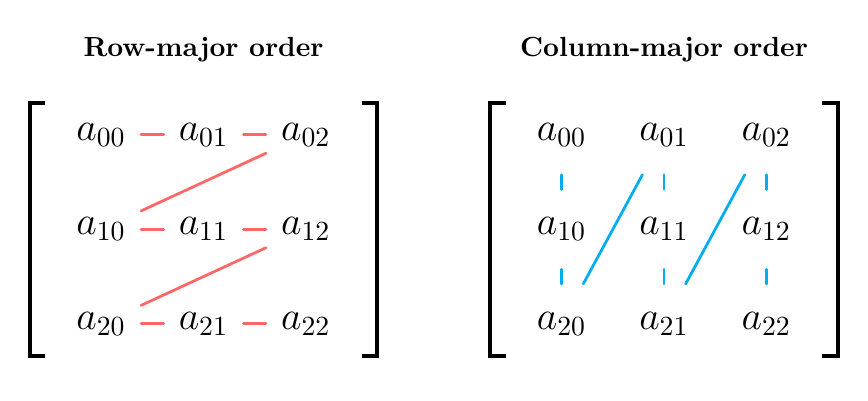
\begin{tikzpicture}[
    % Custom styles for the grids and labels
    matgrid/.style={
        matrix of math nodes,
        nodes={anchor=center, minimum size=1.0cm, font=\Large},
        row sep=0.2cm,
        column sep=0.3cm,
    },
    title/.style={font=\bfseries, align=center},
    % Recreate the specific colors from the reference image
    rm_color/.style={red!60}, % Salmon-red for Row-Major
    cm_color/.style={cyan}  % Cyan for Column-Major
]

% ==========================================
% LEFT: ROW-MAJOR TRAVERSAL
% ==========================================
% 1. The Matrix Grid (inside the brackets)
\matrix (RM) [matgrid] {
    a_{00} & a_{01} & a_{02} \\
    a_{10} & a_{11} & a_{12} \\
    a_{20} & a_{21} & a_{22} \\
};

% 2. The Title (Placed relative to the matrix)
\node[title, above=0.3cm of RM-1-2] (rm_title) {Row-major order};

% 3. The Math Brackets (drawn manually for precision)
\draw[line width=1.5pt] ($(RM-1-1.north west)+(-0.2,-0.1)$) -- ++(-0.2,0) |- ($(RM-3-1.south west)+(-0.2,0.1)$);
\draw[line width=1.5pt] ($(RM-1-3.north east)+(0.2,-0.1)$) -- ++(0.2,0) |- ($(RM-3-3.south east)+(0.2,0.1)$);

% 4. The Path (The Zigzag Line)
% Draw connecting lines between cell anchors
\begin{scope}[rm_color, line width=1pt, line cap=round]
    % Row 1
    \draw (RM-1-1) -- (RM-1-2) -- (RM-1-3);
    % Row 2 Jump and Sweep
    \draw (RM-1-3) -- (RM-2-1);
    \draw (RM-2-1) -- (RM-2-2) -- (RM-2-3);
    % Row 3 Jump and Sweep
    \draw (RM-2-3) -- (RM-3-1);
    \draw (RM-3-1) -- (RM-3-2);
    % Final arrow segment, offset slightly from the last element a33
    \draw (RM-3-2) -- (RM-3-3);
\end{scope}

% ==========================================
% RIGHT: COLUMN-MAJOR TRAVERSAL
% ==========================================
% 1. The Matrix Grid (Placed right of the first matrix)
\matrix (CM) [matgrid, right=2.0cm of RM] {
    a_{00} & a_{01} & a_{02} \\
    a_{10} & a_{11} & a_{12} \\
    a_{20} & a_{21} & a_{22} \\
};

% 2. The Title (Placed relative to the matrix)
\node[title, above=0.3cm of CM-1-2] (cm_title) {Column-major order};

% 3. The Math Brackets (drawn manually)
\draw[line width=1.5pt] ($(CM-1-1.north west)+(-0.2,-0.1)$) -- ++(-0.2,0) |- ($(CM-3-1.south west)+(-0.2,0.1)$);
\draw[line width=1.5pt] ($(CM-1-3.north east)+(0.2,-0.1)$) -- ++(0.2,0) |- ($(CM-3-3.south east)+(0.2,0.1)$);

% 4. The Path (The N-shape Lines)
\begin{scope}[cm_color, line width=1pt, line cap=round]
    % Col 1
    \draw (CM-1-1) -- (CM-2-1) -- (CM-3-1);
    % Col 2 Jump and Sweep
    \draw (CM-3-1) -- (CM-1-2);
    \draw (CM-1-2) -- (CM-2-2) -- (CM-3-2);
    % Col 3 Jump and Sweep
    \draw (CM-3-2) -- (CM-1-3);
    \draw (CM-1-3) -- (CM-2-3);
    % Final arrow segment, offset from a33
    \draw (CM-2-3) -- (CM-3-3);
\end{scope}

\end{tikzpicture}

\end{figure}

This implementation chooses row-major as the data representation for our matrices. The index of the element $a_{i,j}$ of
an $n\times m$ matrix $A$ in the row-major array representing the matrix is $im + j$.

We can implement a basic matrix multiplication algorithm based on the dot-product formulation from Definition \ref{def:mat-mul}.

\begin{lstlisting}[mathescape=true]
function multiply(Matrix<n,m> X, Matrix<m,p> Y) {
  Matrix<n,p> V;

  for (i : [0,...,n-1]) {
    for (j : [0,...,p-1]) {
      int sum = $-\infty$;
      for (k : [0,...,m-1]) {
        sum = max(sum, X[i,k] + Y[k,j]);
      }
      V[i,j] = sum;
    }
  }

  return V;
}
\end{lstlisting}

Modern CPU caching exploits spatial locality of reference, where if a piece of data is accessed by the CPU, other pieces
of data in close proximity will be in the same cache line or prefetched into the cache, therefore reducing the chance of
an expensive cache miss.
In the chosen algorithm, matrices X and Y are both stored in row-major order, yet inside the inner loop, X is being accessed in
row-major order, and Y is being accessed in column-major order. The elements of Y being accessed on consecutive iterations 
are not in close proximity to each other in memory, and so cache misses dominate the running time, rather than the 
actual calculations.

This issue can be avoided by storing matrices in both row-major and column-major order. Then, depending on whether the
matrix is the right or left operand in a multiplication, we can select the most cache-friendly option to traverse.
This however, doubles our memory usage, and so we instead try to change the order in which we access elements of the matrices.

\subsection{Traversal order and cache performance}

The three loops in the previous matrix multiplication can be arbitrarily swapped with each other without an effect 
on correctness or asymptotic running time. We can swap our $k$ and $j$ loops so that the inner loop traverses Y in 
row-major order, resulting in the following algorithm:

\begin{lstlisting}[mathescape=true]
function multiply(Matrix<n,m> X, Matrix<m,p> Y) {
  Matrix<n,p> V;

  for (i : [0,...,n-1]) {
    for (k : [0,...,m-1]) {
      int xVal = X[i,k];
      if (xVal == $-\infty$) continue;

      for (j : [0,...,p-1]) {
        V[i,j] = max(V[i,j], xVal + Y[k,j]);
      }
    }
  }

  return V;
}
\end{lstlisting}

Apart from the improved cache performance, there are three other optimisations.

\begin{description}
  \item[Value hoisting] Since the indices $i$ and $k$ do not change in the inner loop of the algorithm, we can hoist the 
    retrieval of $X_{i,k}$ outside of the loop.
  \item[Sparsity] This optimisation concerns line 7 of the algorithm. To make sense of it, we can consider an extension
    to the previous matrix multiplication definition:
    $$
    v_{i \cdot} = \displaystyle\sum_{k=1}^{n} \! {}_{\oplus} x_{ik} \odot y_{k\cdot}
    $$
    This says that the $i$th row of $V$ is a linear combination of the $k$ rows of $Y$. More importantly, note that 
    $$
    -\infty \odot
    \begin{bmatrix}
      y_{k 1} \\
      \vdots \\
      y_{k p}
    \end{bmatrix}
    =
    \begin{bmatrix}
      -\infty \\ 
      \vdots \\ 
      -\infty
    \end{bmatrix}
    $$
    and since $-\infty$ is the additive identity, this row does not contribute to the final sum, and so the dot product 
    can be skipped. So, more precisely, the $i$th row of $V$ is a linear combination of the $k$ rows of $Y$ for which 
    $x_{ik}$ is not $-\infty$ \cite{gustavson-sparse}. The matrices in this project tend to be fairly sparse and so this 
    results in a significant performance improvement.
  \item[Vectorisation] Finally, since $Y$ is traversed contiguously in the inner loop, this makes it easily open to 
    optimisations using vector instructions. Vector instructions, also known as SIMD (Single-Instruction, Multiple-Data) \cite{flynntaxonomy},
    perform the same operation on several operands, exploiting data-level parallelism. The max and addition operations can 
    then be performed on the adjacent data from several iterations of the inner loop using vectorised variants, increasing 
    the number of elements processed per iteration.
\end{description}

\subsection{Matrix tiling}

%TODO: Do i need a more in-depth explanation?

One other common method of improving the cache performance of matrix multiplication algorithms is \textit{tiling}.
This involves implicitly dividing the matrix into square tiles of smaller sizes, and instead of traversing an entire 
row and column of the operands in one sweep to compute a cell of the output matrix, the algorithm works only on the values 
within one tile, before moving onto the next. This improves the spatial locality of memory accesses, as elements at the 
beginning of a row are not evicted by the time we get to the end of the row, which is a problem for large matrices.

However, since we are only tracking register dependencies in this project, our matrices are only approximately $64 \times 64$
in size. Assuming each cell holds a 32-bit integer, an entire matrix is stored in $64\cdot 64 \cdot 4 =16384$ bytes, 
which can be easily held in the 32 or 64KiB L1 cache of a modern processor core.

In this case, tiling the matrix will actually result in unnecessary overhead from a more complex control flow.

\subsection{Sparse Matrices}



%TODO: Diagram


\subsubsection{CSR Matrix Format}




\subsubsection{Sparse Matrix Multiplication}

\section{Expression Reduction}

\subsection{Fast exponentiation}

Can do fast exponentiation logarithmically. However repetitions usually happen on the loop level, not on the instruction level, so we need to first shrink the representation of a loop into a single matrix.

\subsection{Pair-reduction}

An approach that ends up reducing loops into a single matrix is a general one - memoisation.

%TODO: #check fixed point
This leads to an iterative (FIXED POINT? ) computation, where at each iteration, we select a pair of matrices to compute their product. We then cache that value, and scan through the entire expression, replacing every instance of that pair with the computed result. After that pass, we look for any exponents in the expression to reduce logarithmically.

At each iteration, we will shrink a pair of matrices in all iterations of a loop's body into a single matrix. So, after several iterations, the loop's body will be shrunk into a singular matrix, and then we can leverage logarithmic exponentiation to quickly shrink the repeated loop matrices into a single matrix.
%TODO: #todo include diagram demonstrating

We want to make sure that we make the most cost-effective multiplication at each iteration. Clearly we save the most cost by making the most frequent calculation in the matrix. 
To ensure this, we iterate through the expression, and select the most frequent pair of them all.
%TODO: #clarify on why we absolutely need this! see below para.

This also has the side-effect of reducing common pairs of instructions quickly through memoisation of the result. 

Once the frequency of the most frequent pair is 1, we can safely continue to directly multiplying matrices (as now there is no point in memoising values or doing frequency computations).

%TODO: todo add pseudocode

\subsection{Multiple pair-reduction}

*while the single-pair reduction ensures the minimum number of multiplications are made, frequency calculation is expensive. As the algorithm progresses, the frequency of pairs tends to reduce, and so the cost of the frequency calculation rises in comparison to the cost saved by memoising the most frequent pair.
We can make a tradeoff, replacing more pairs per iteration, which means we make less iterations and less frequency calculations*  %TODO: #rewrite 

*doesn't respect loop structure/why it doesn't ensure minimum number of multiplications*

Consider cksum's inner loop of instructions. They form a 7-instruction cycle, repeating 65536 times, that looks something like this:
$$
(A B C D E F G)^{65536}
$$
Now run the expression reduction, replacing the top 8 most frequent pairs:
%TODO: #todo add drawn diagram
We can see that we have reduced two iterations of the loop into one cycle of 7 matrices repeating 32768 times.
Since this is not exponentiation of one singular matrix, we cannot reduce this using logarithmic exponentiation, and instead have to go through more iterations of frequency computation and pair reductions (at each iteration halving the exponent) until we end up with a single loop of 7 matrices with an exponent of 1.
%TODO: #justify do the maths on which is better ^^^ #rewrite 
We haven't respected the boundaries of the loop and therefore haven't reduced INSIDE the loop

%TODO: #todo variable N-pair processing!!!

We want to exploit both the optimal reduction of replacing fewer pairs per iteration, and the increased throughput of replacing more pairs.
Because of our frequency-based approach, loop bodies shrink earlier (as the body's instructions occur many times!). Once the loops are reduced, we then have lower frequency values which we want to deal with by reducing more pairs every iteration.
We can do this by increasing the number of pairs to replace each iteration. How to do this, I am unsure as I haven't actually implemented any code. How silly of me.

%TODO: #todo analysis of how equation size changes with paircount

\subsection{Block preprocessing}

In the data given to us we can actually see branch structure so we reduce with respect to loops better - some loops occur over many different branches - this doesn't help here.

\subsection{Finding loops}

\section{Thread-level parallelism}

\section{Accelerator Compute}



\chapter{Evaluation}

I evaluated the following cool thing...

The pair encoding scheme still does significant work reduction after the loop finder runs, showing there is more general 
redundancy 

\section{Methodology}

Talk about how results were acquired

\section{Algorithmic and data-driven optimisations}

\begin{figure}[htbp]
  \centering
  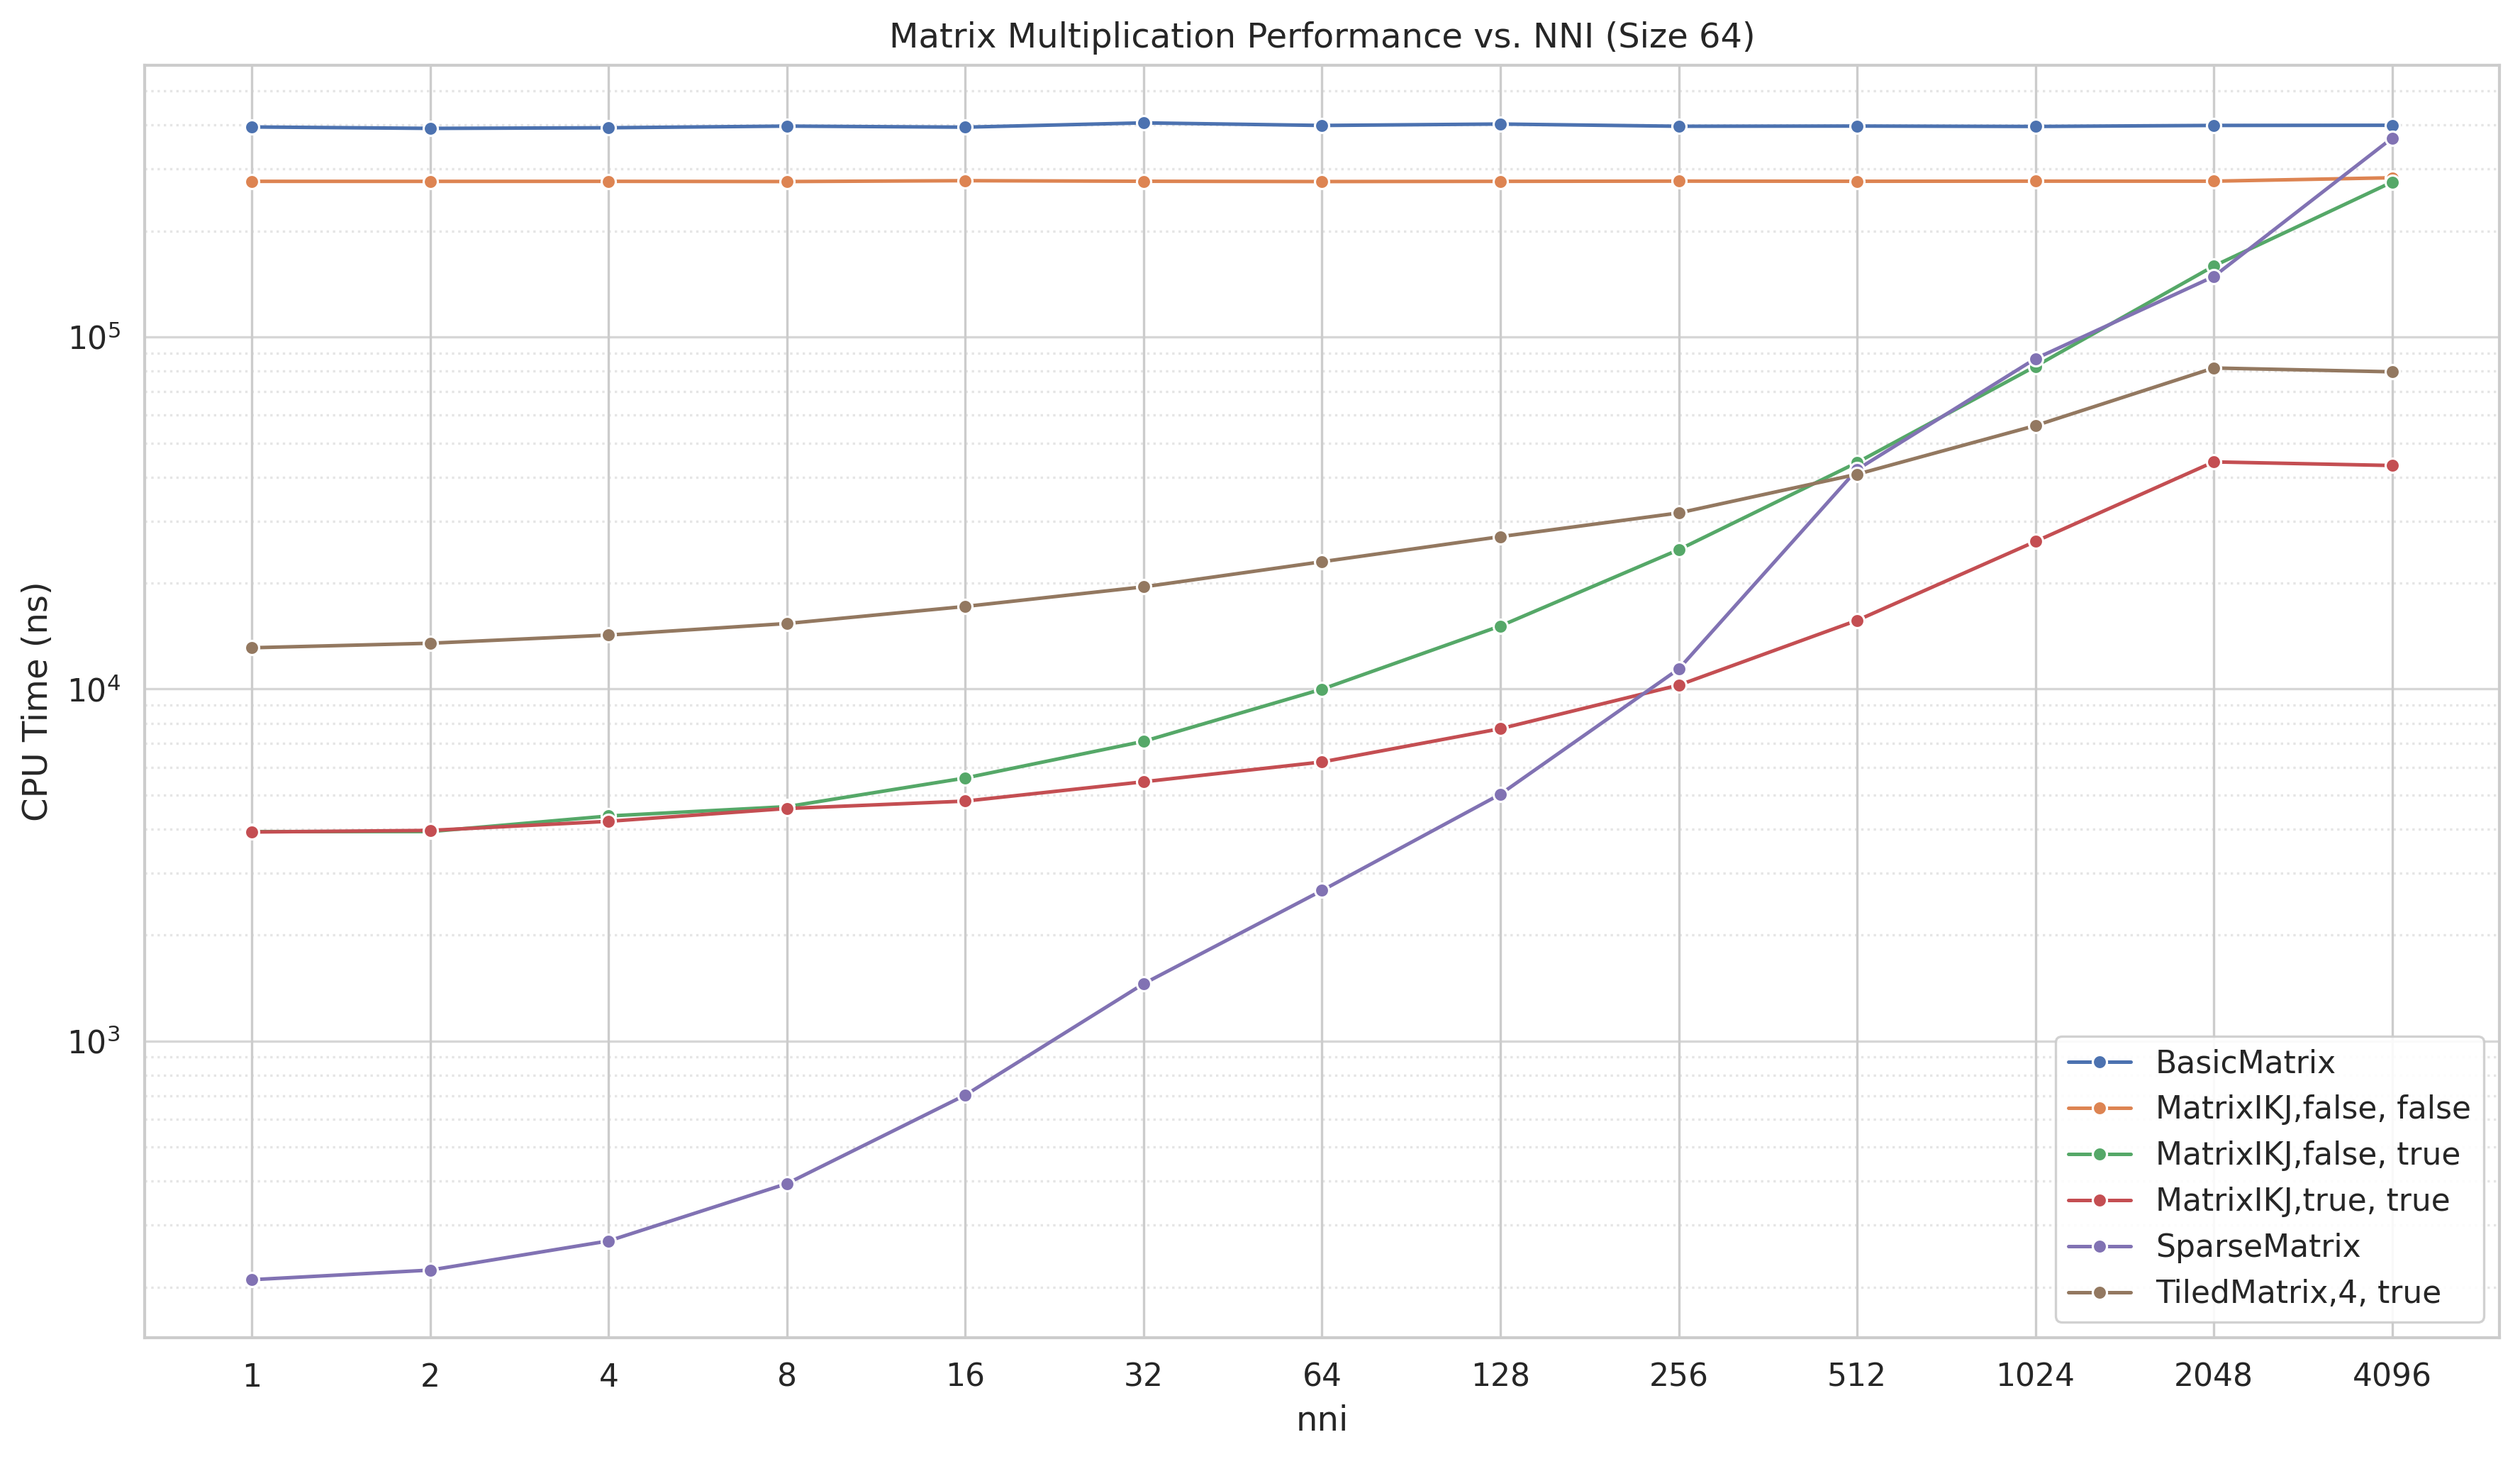
\includegraphics[width=0.5\textwidth]{graphs/matrix_nni_performance.png}
  \caption{Comparing runtime of matrix multiplication approaches, for matrices of varying sparsity.}
  \label{eval:fig:matrix-perf}
\end{figure}

Parameter sweet spots for encoding - minimise parameters 

\begin{figure}[htbp]
  \centering
  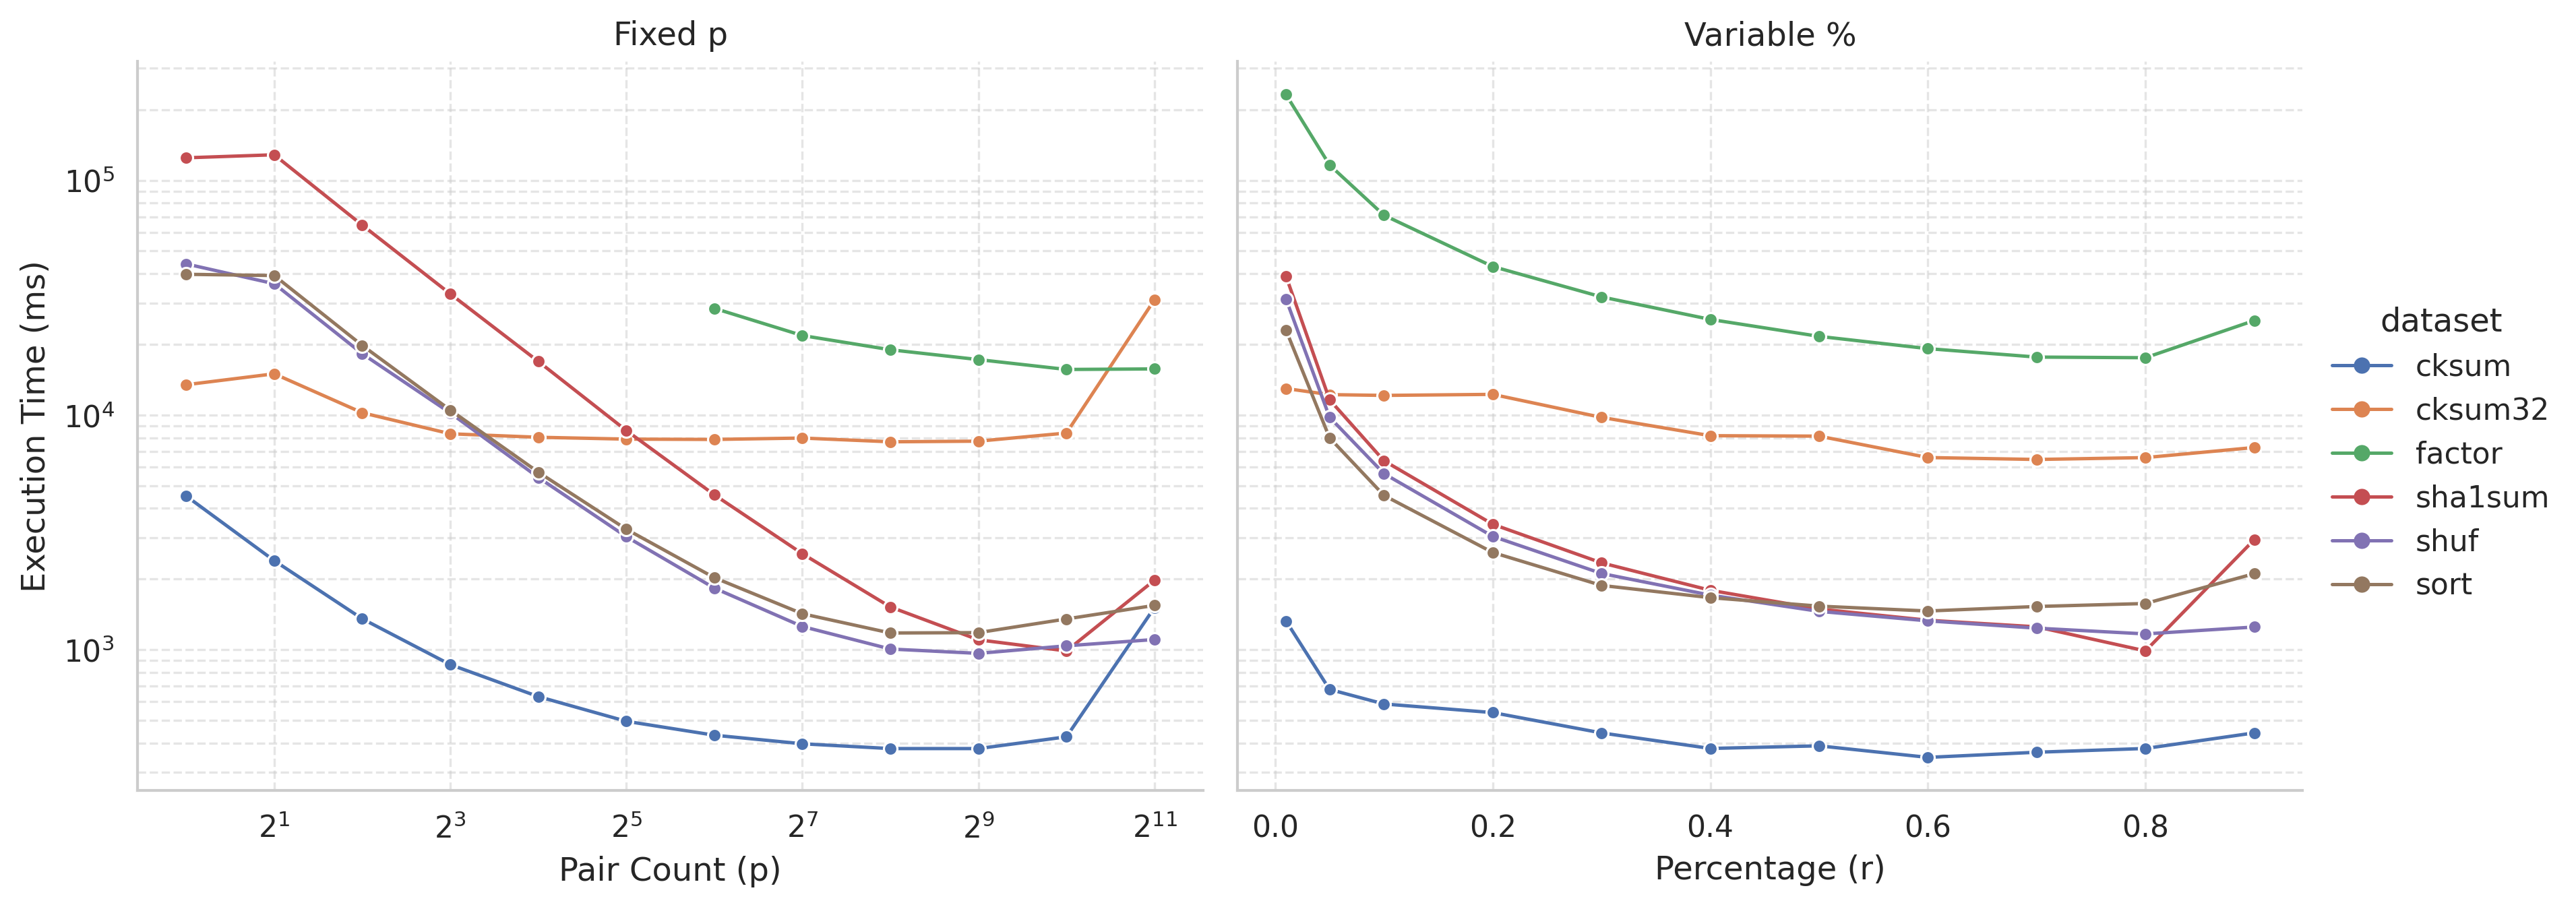
\includegraphics[width=0.8\textwidth]{graphs/encoder_time.png}
  \caption{Comparing runtime of program on different datasets, for different encoder parameters, excluding block 
  preprocessing and loop finding.}
  \label{eval:fig:encoder-perf}
\end{figure}

\begin{figure}[htbp]
  \centering
  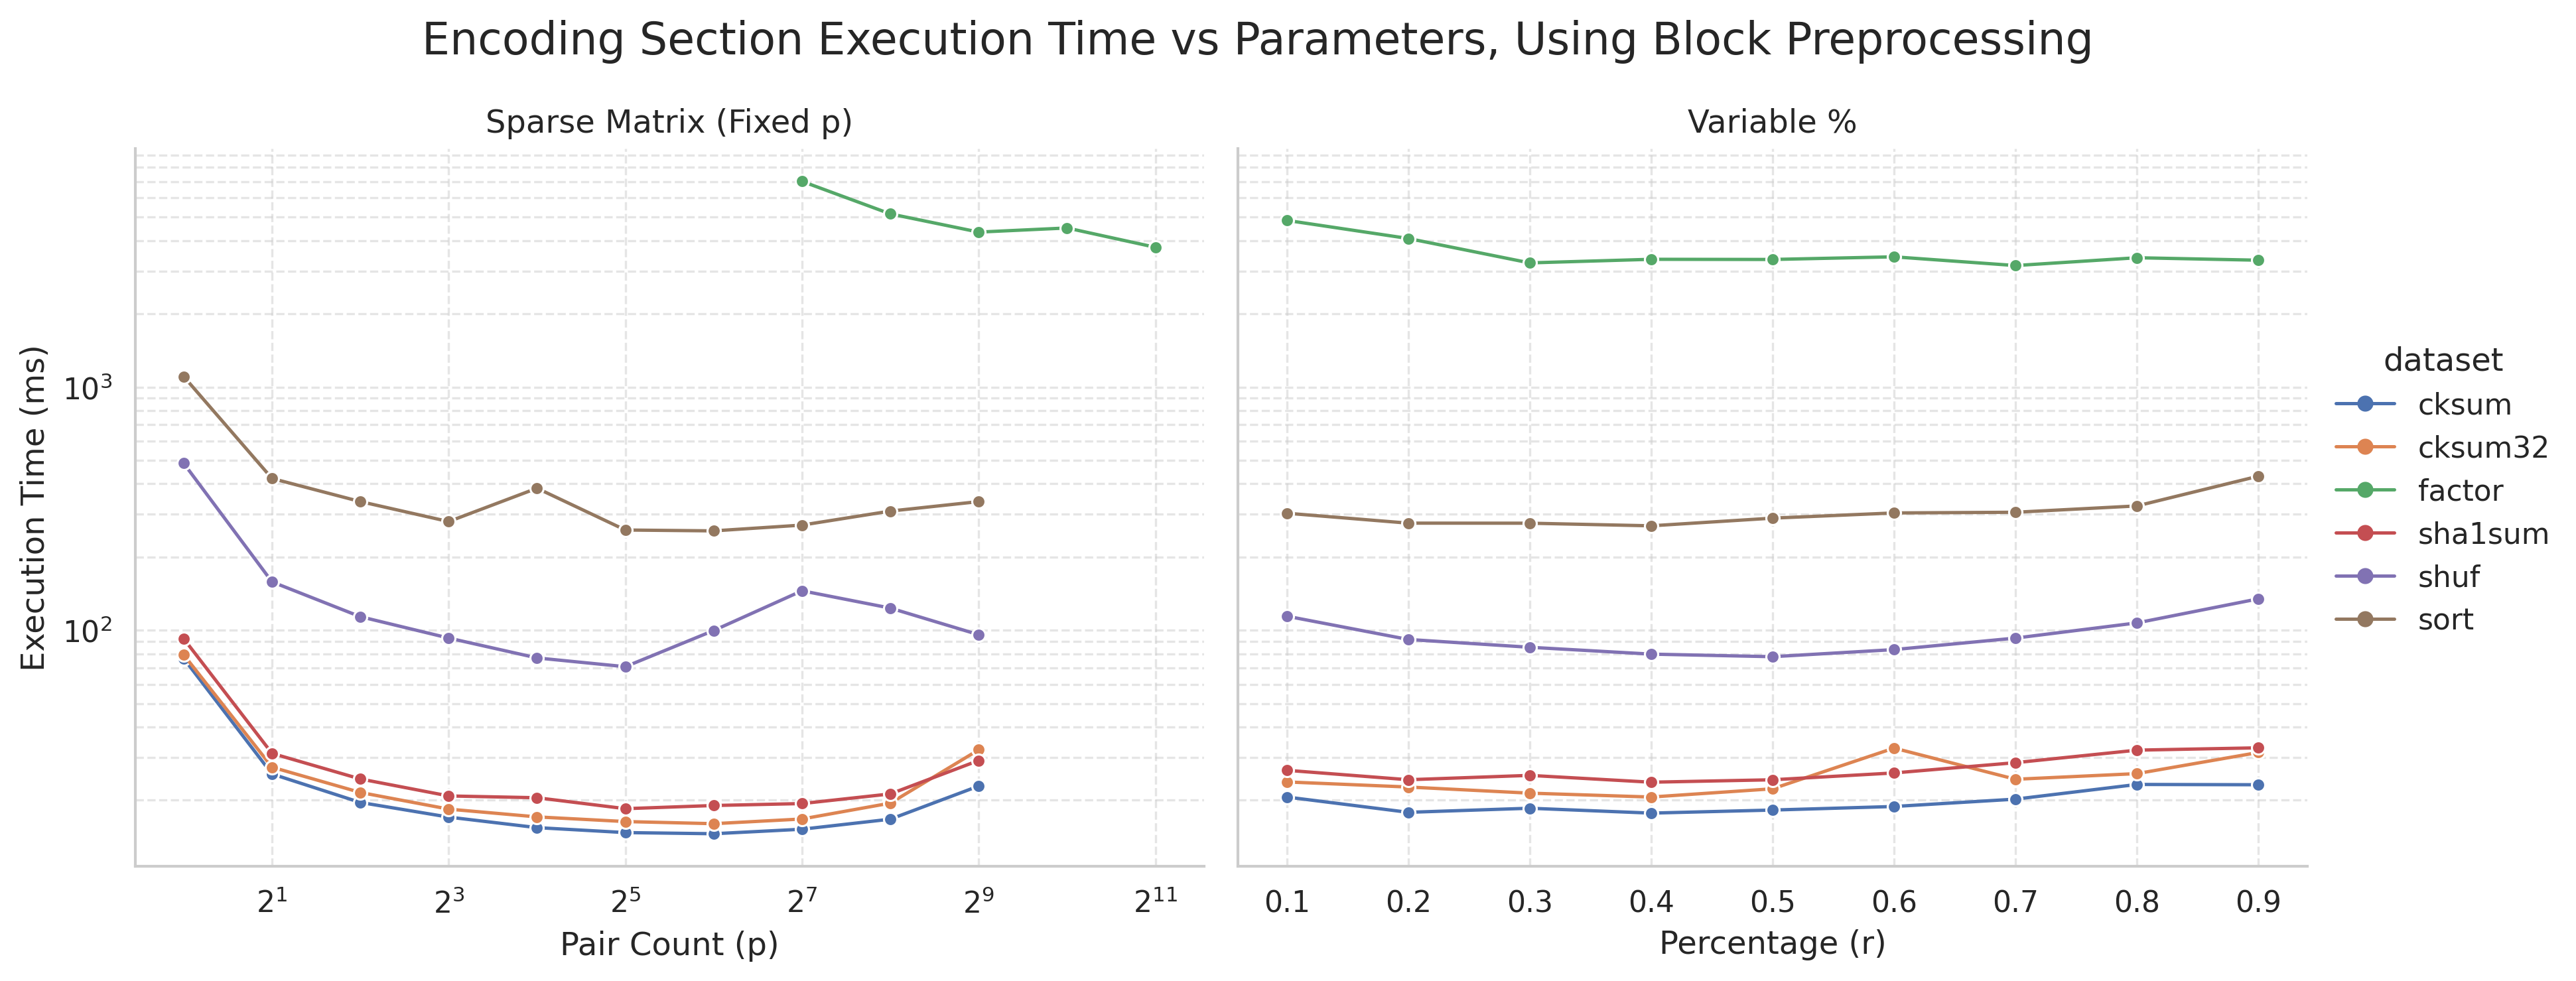
\includegraphics[width=0.8\textwidth]{graphs/encoder_time_block.png}
  \caption{Comparing runtime of program on different datasets, for different encoder parameters, including block 
  preprocessing.}
  \label{eval:fig:encoder-block-perf}
\end{figure}

\begin{figure}[htbp]
  \centering
  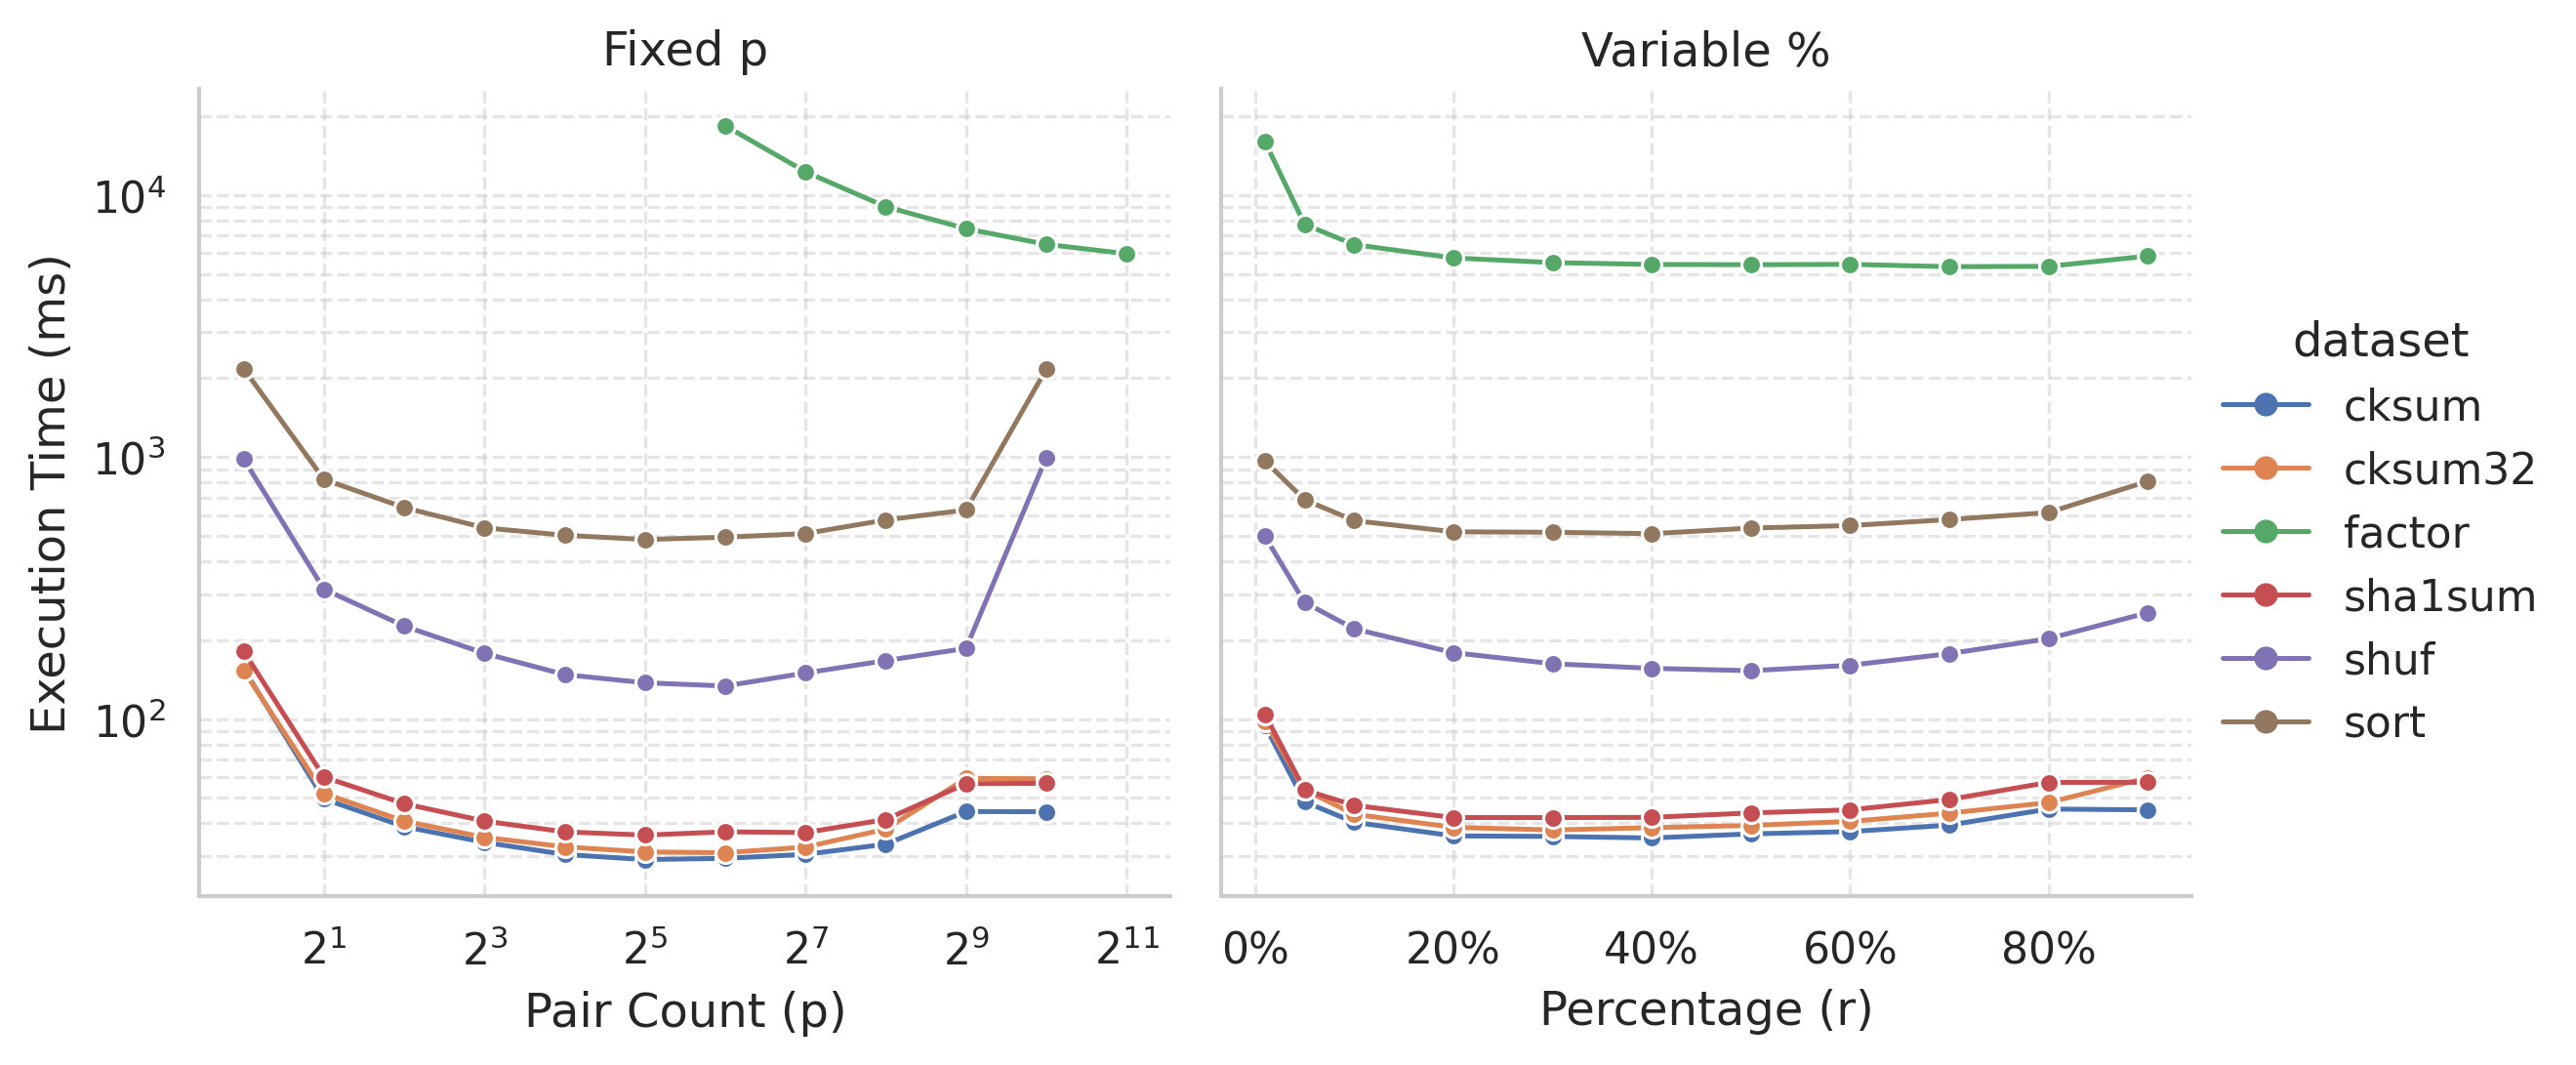
\includegraphics[width=0.8\textwidth]{graphs/encoder_time_loop.png}
  \caption{Comparing runtime of program on different datasets, for different encoder parameters, including block 
  preprocessing and loop finding.}
  \label{eval:fig:encoder-block-loop-perf}
\end{figure}

Compression ratio for encoders.

\begin{figure}[htbp]
  \centering
  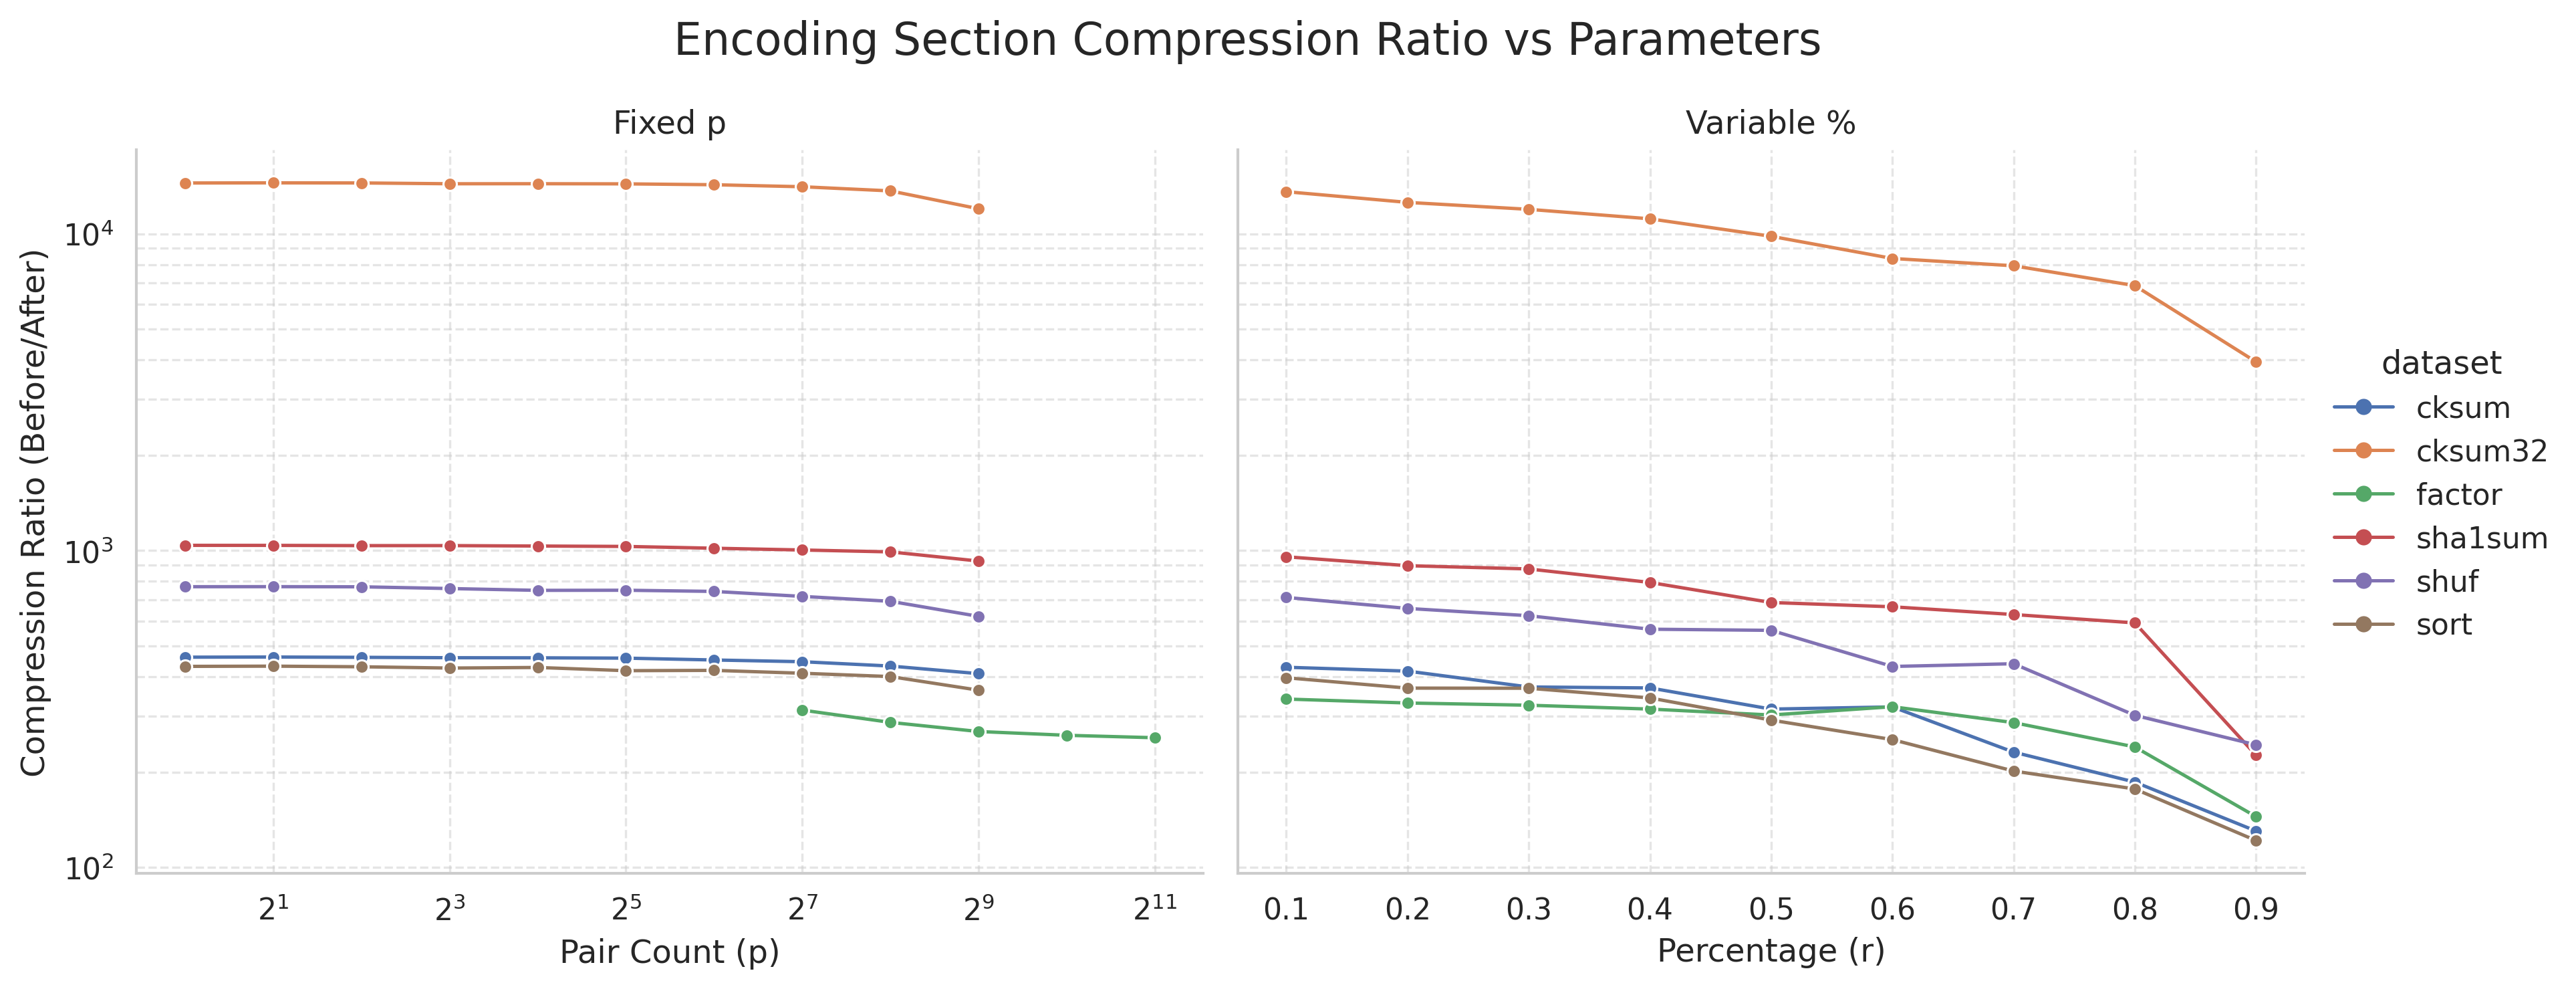
\includegraphics[width=0.8\textwidth]{graphs/encoder_compression.png}
  \caption{Comparing compression ratio of encoder on different datasets, for different encoder parameters, excluding block 
  preprocessing and loop finding.}
  \label{eval:fig:encoder-comp}
\end{figure}

\begin{figure}[htbp]
  \centering
  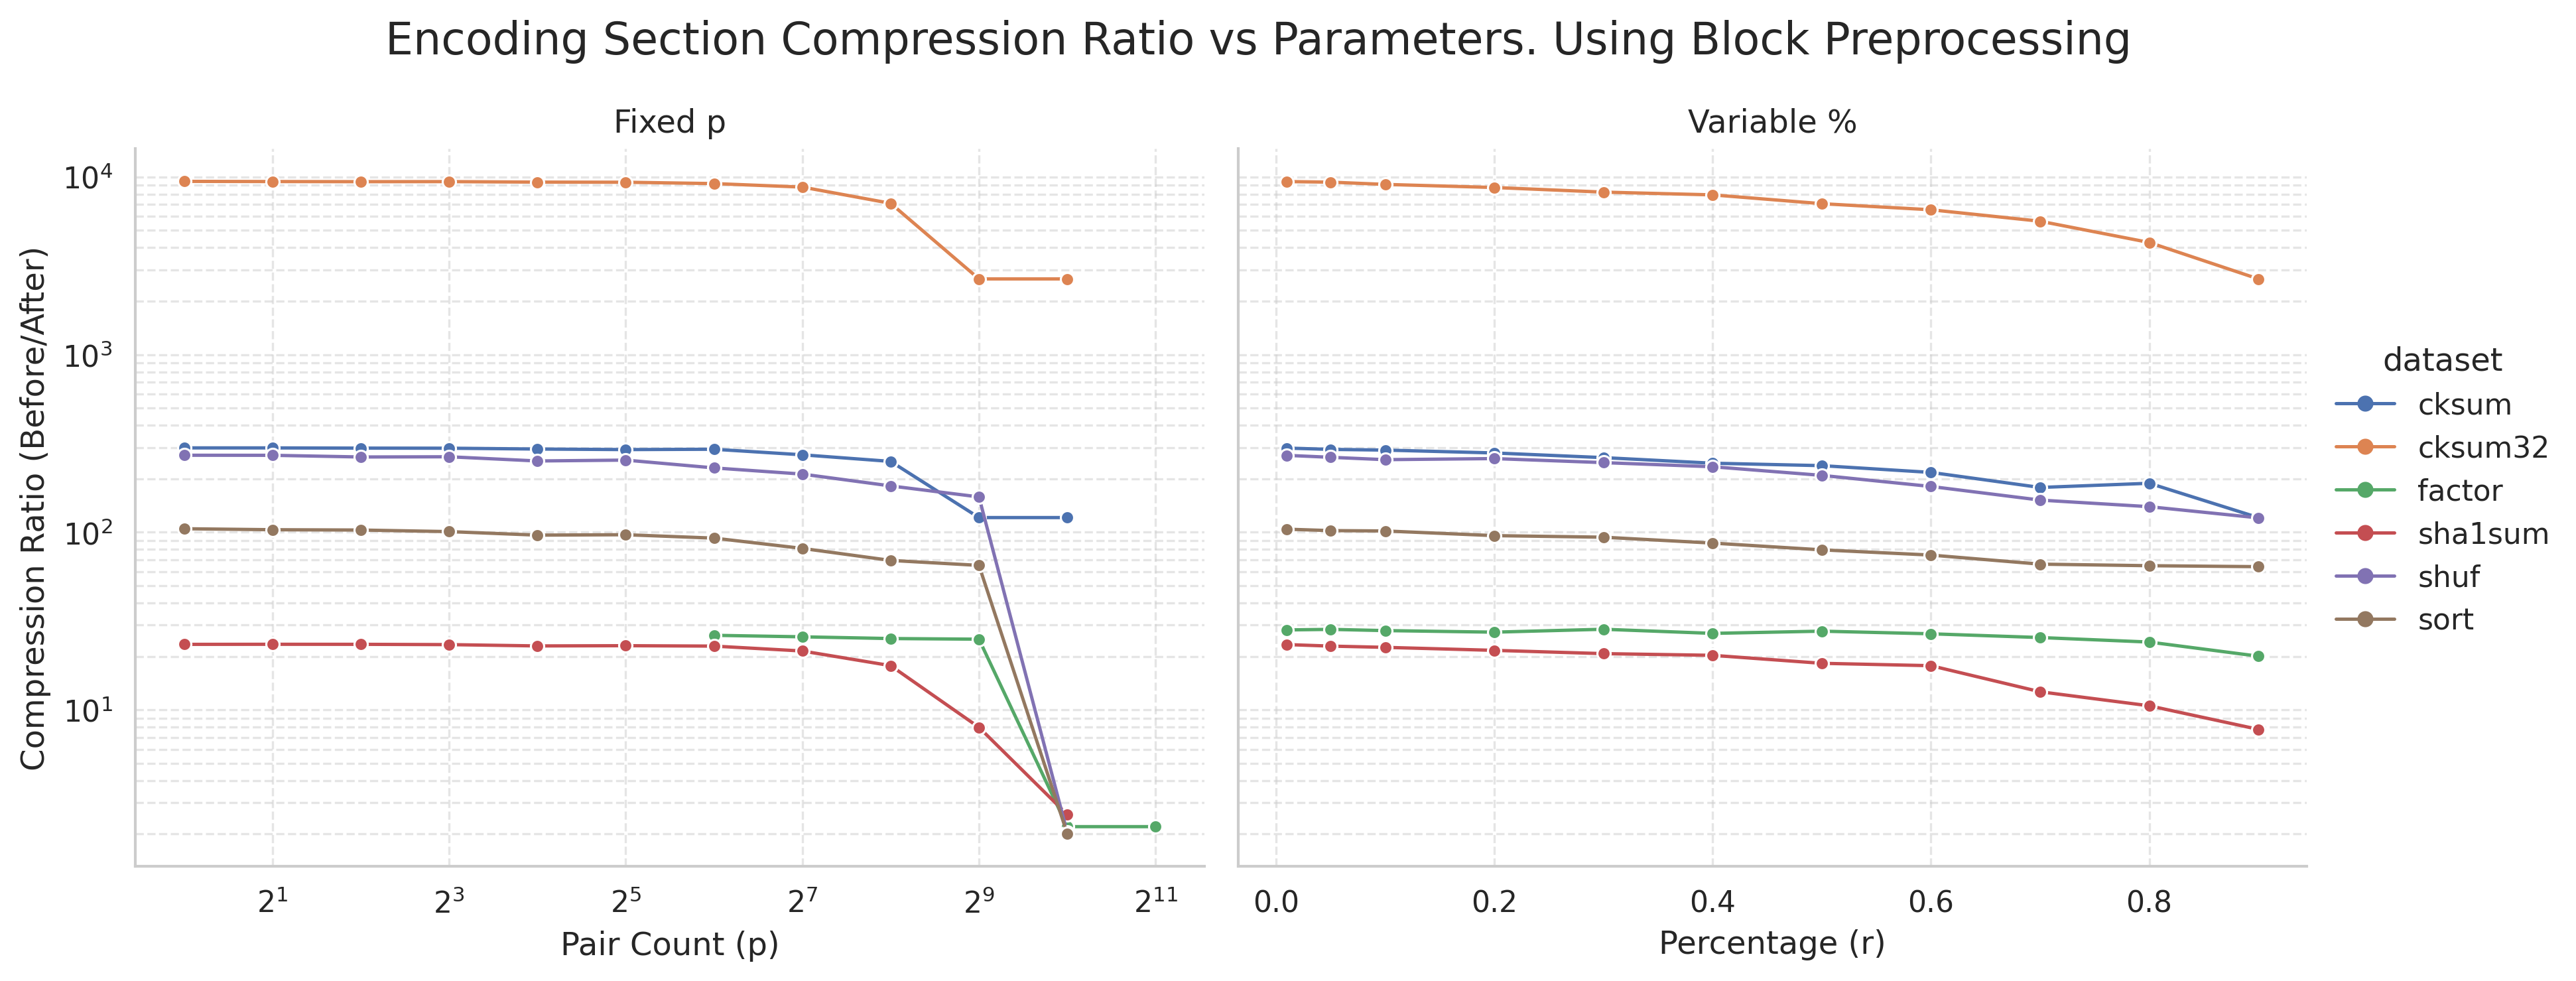
\includegraphics[width=0.8\textwidth]{graphs/encoder_compression_block.png}
  \caption{Comparing runtime of program on different datasets, for different encoder parameters, including block 
  preprocessing.}
  \label{eval:fig:encoder-block-comp}
\end{figure}

\begin{figure}[htbp]
  \centering
  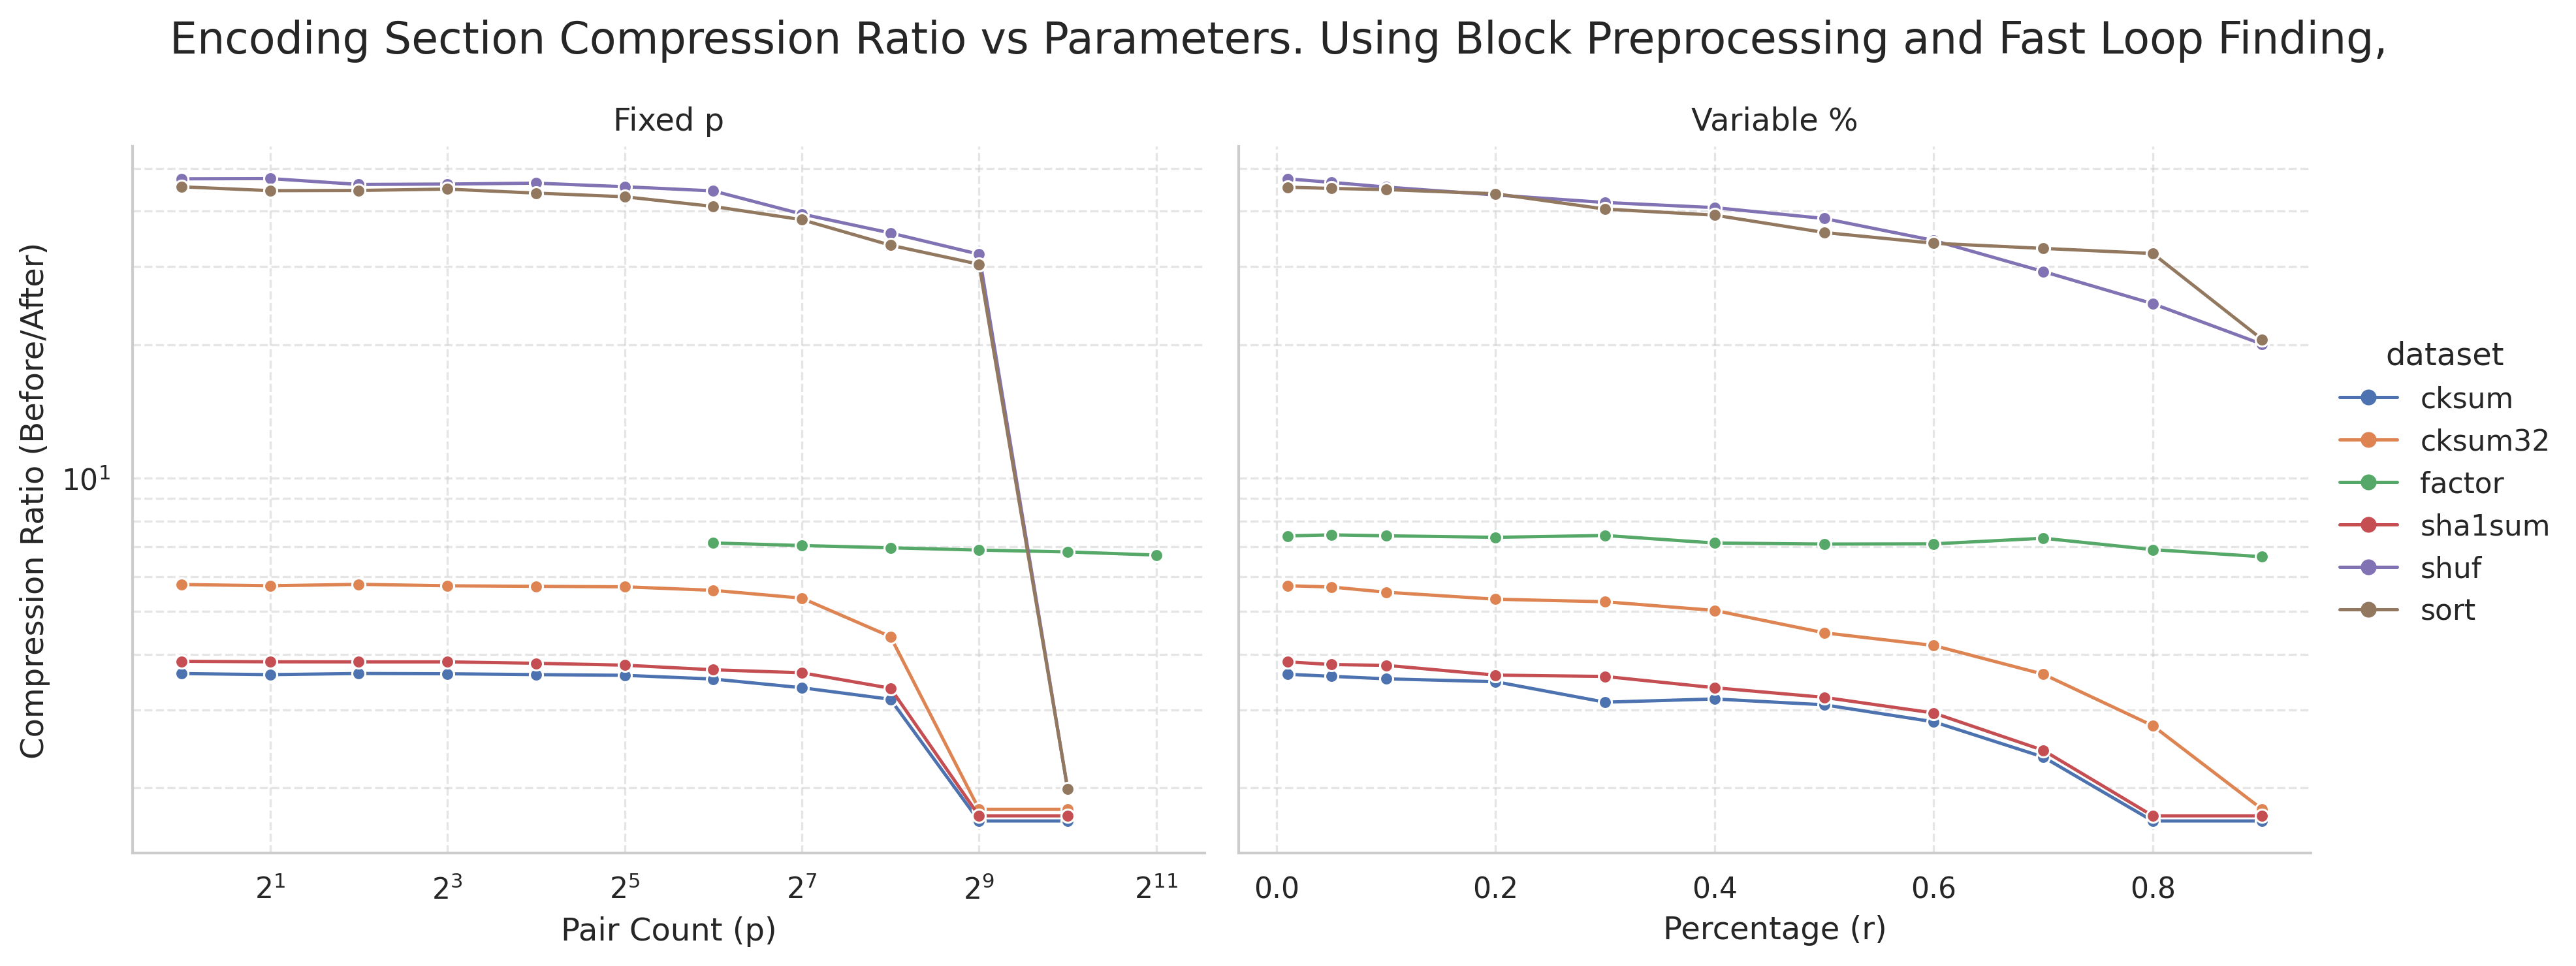
\includegraphics[width=0.8\textwidth]{graphs/encoder_compression_loop.png}
  \caption{Comparing runtime of program on different datasets, for different encoder parameters, including block 
  preprocessing and loop finding.}
  \label{eval:fig:encoder-block-loop-comp}
\end{figure}

expression size vs iteration

\begin{figure}[htbp]
  \centering
  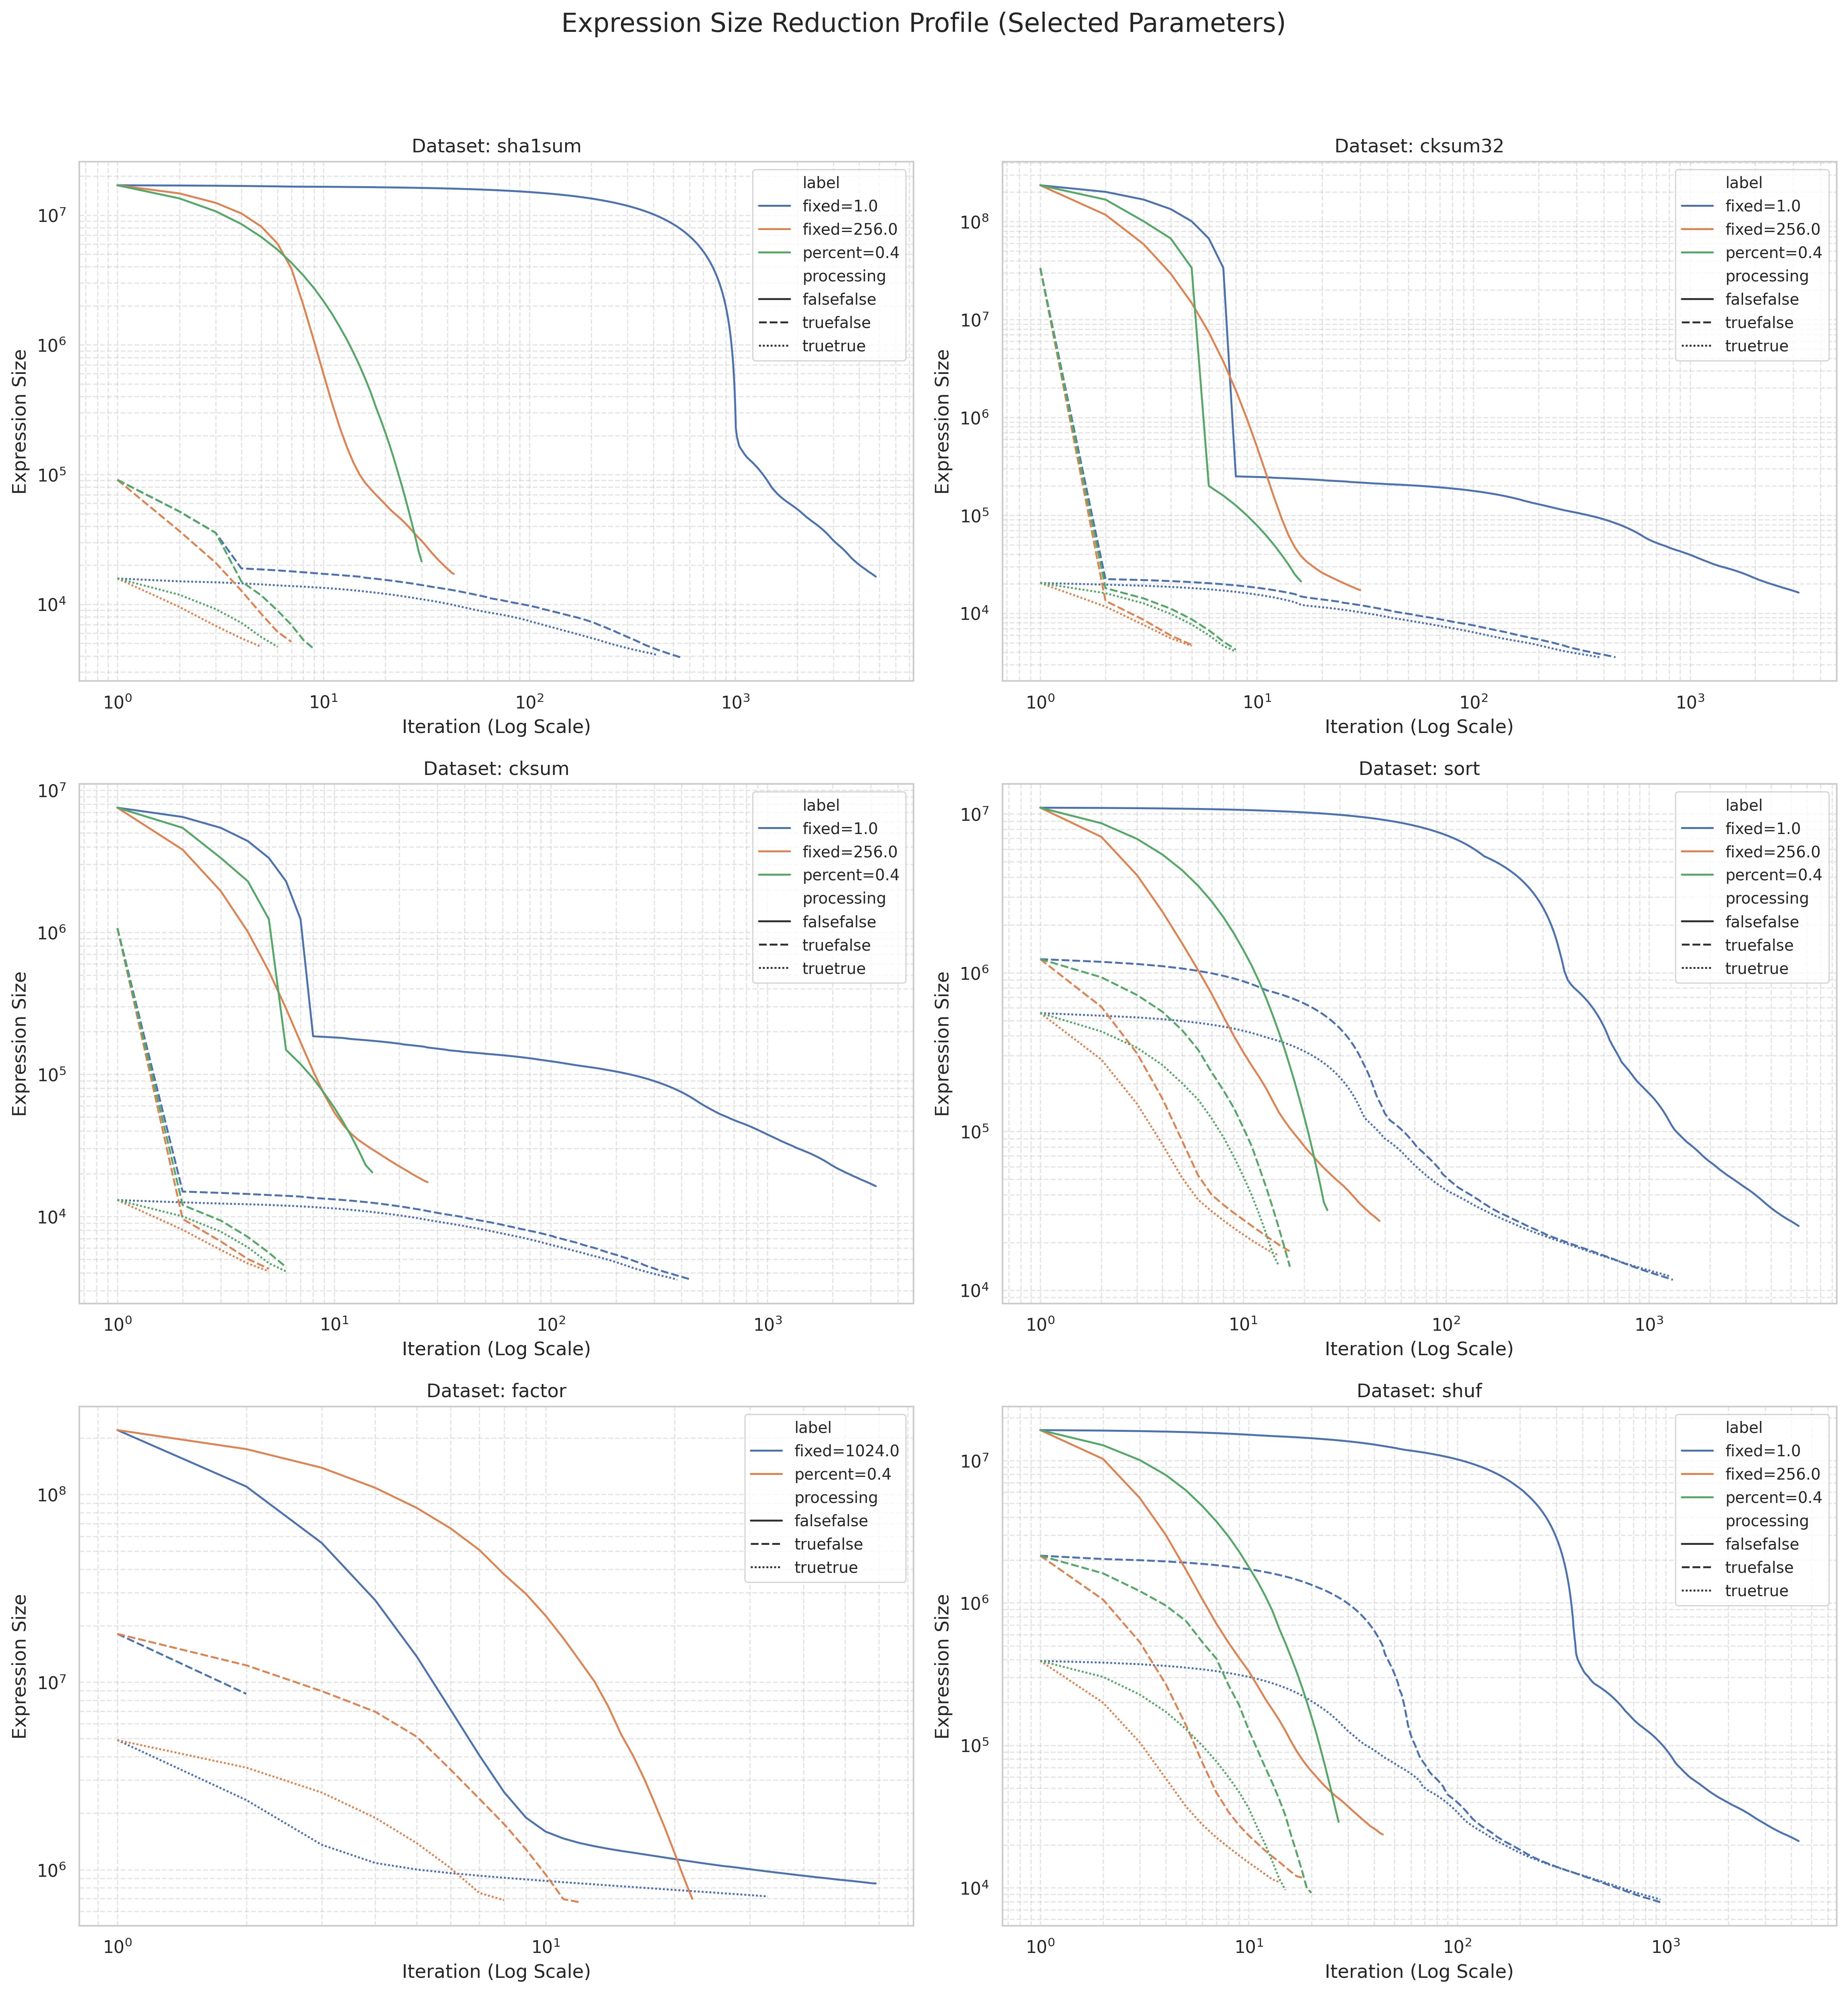
\includegraphics[width=1\textwidth]{graphs/encoder_profile.png}
  \caption{Comparing reduction behaviour of encoder on different datasets, for representative parameters.}
  \label{eval:fig:encoder-profile}
\end{figure}

Table for mults vs iterations for no processing, block processing, loop finding

\begin{table}[ht]
\begin{center}
\begin{tabular}{lcccc}
  \textbf{Dataset} & \textbf{Blocks} & \textbf{Fast Loops} & \textbf{Multiplications} & \textbf{Iterations} \\
  \midrule
  cksum \\
  cksum \\
  cksum \\
  cksum32\\
  cksum32\\
  cksum32\\
  factor\\
  factor\\
  factor\\
  sha1sum\\
  sha1sum\\
  sha1sum\\
  shuf \\
  shuf \\
  shuf \\
  sort\\
  sort\\
  sort\\
  \midrule
\end{tabular}
\end{center}
\caption{Summary of total multiplications and encoder iterations on the selected data.}
\label{tbl:single-thread-mults}
\end{table}

time tradeoff for each pipeline component

\begin{figure}[htbp]
  \centering
  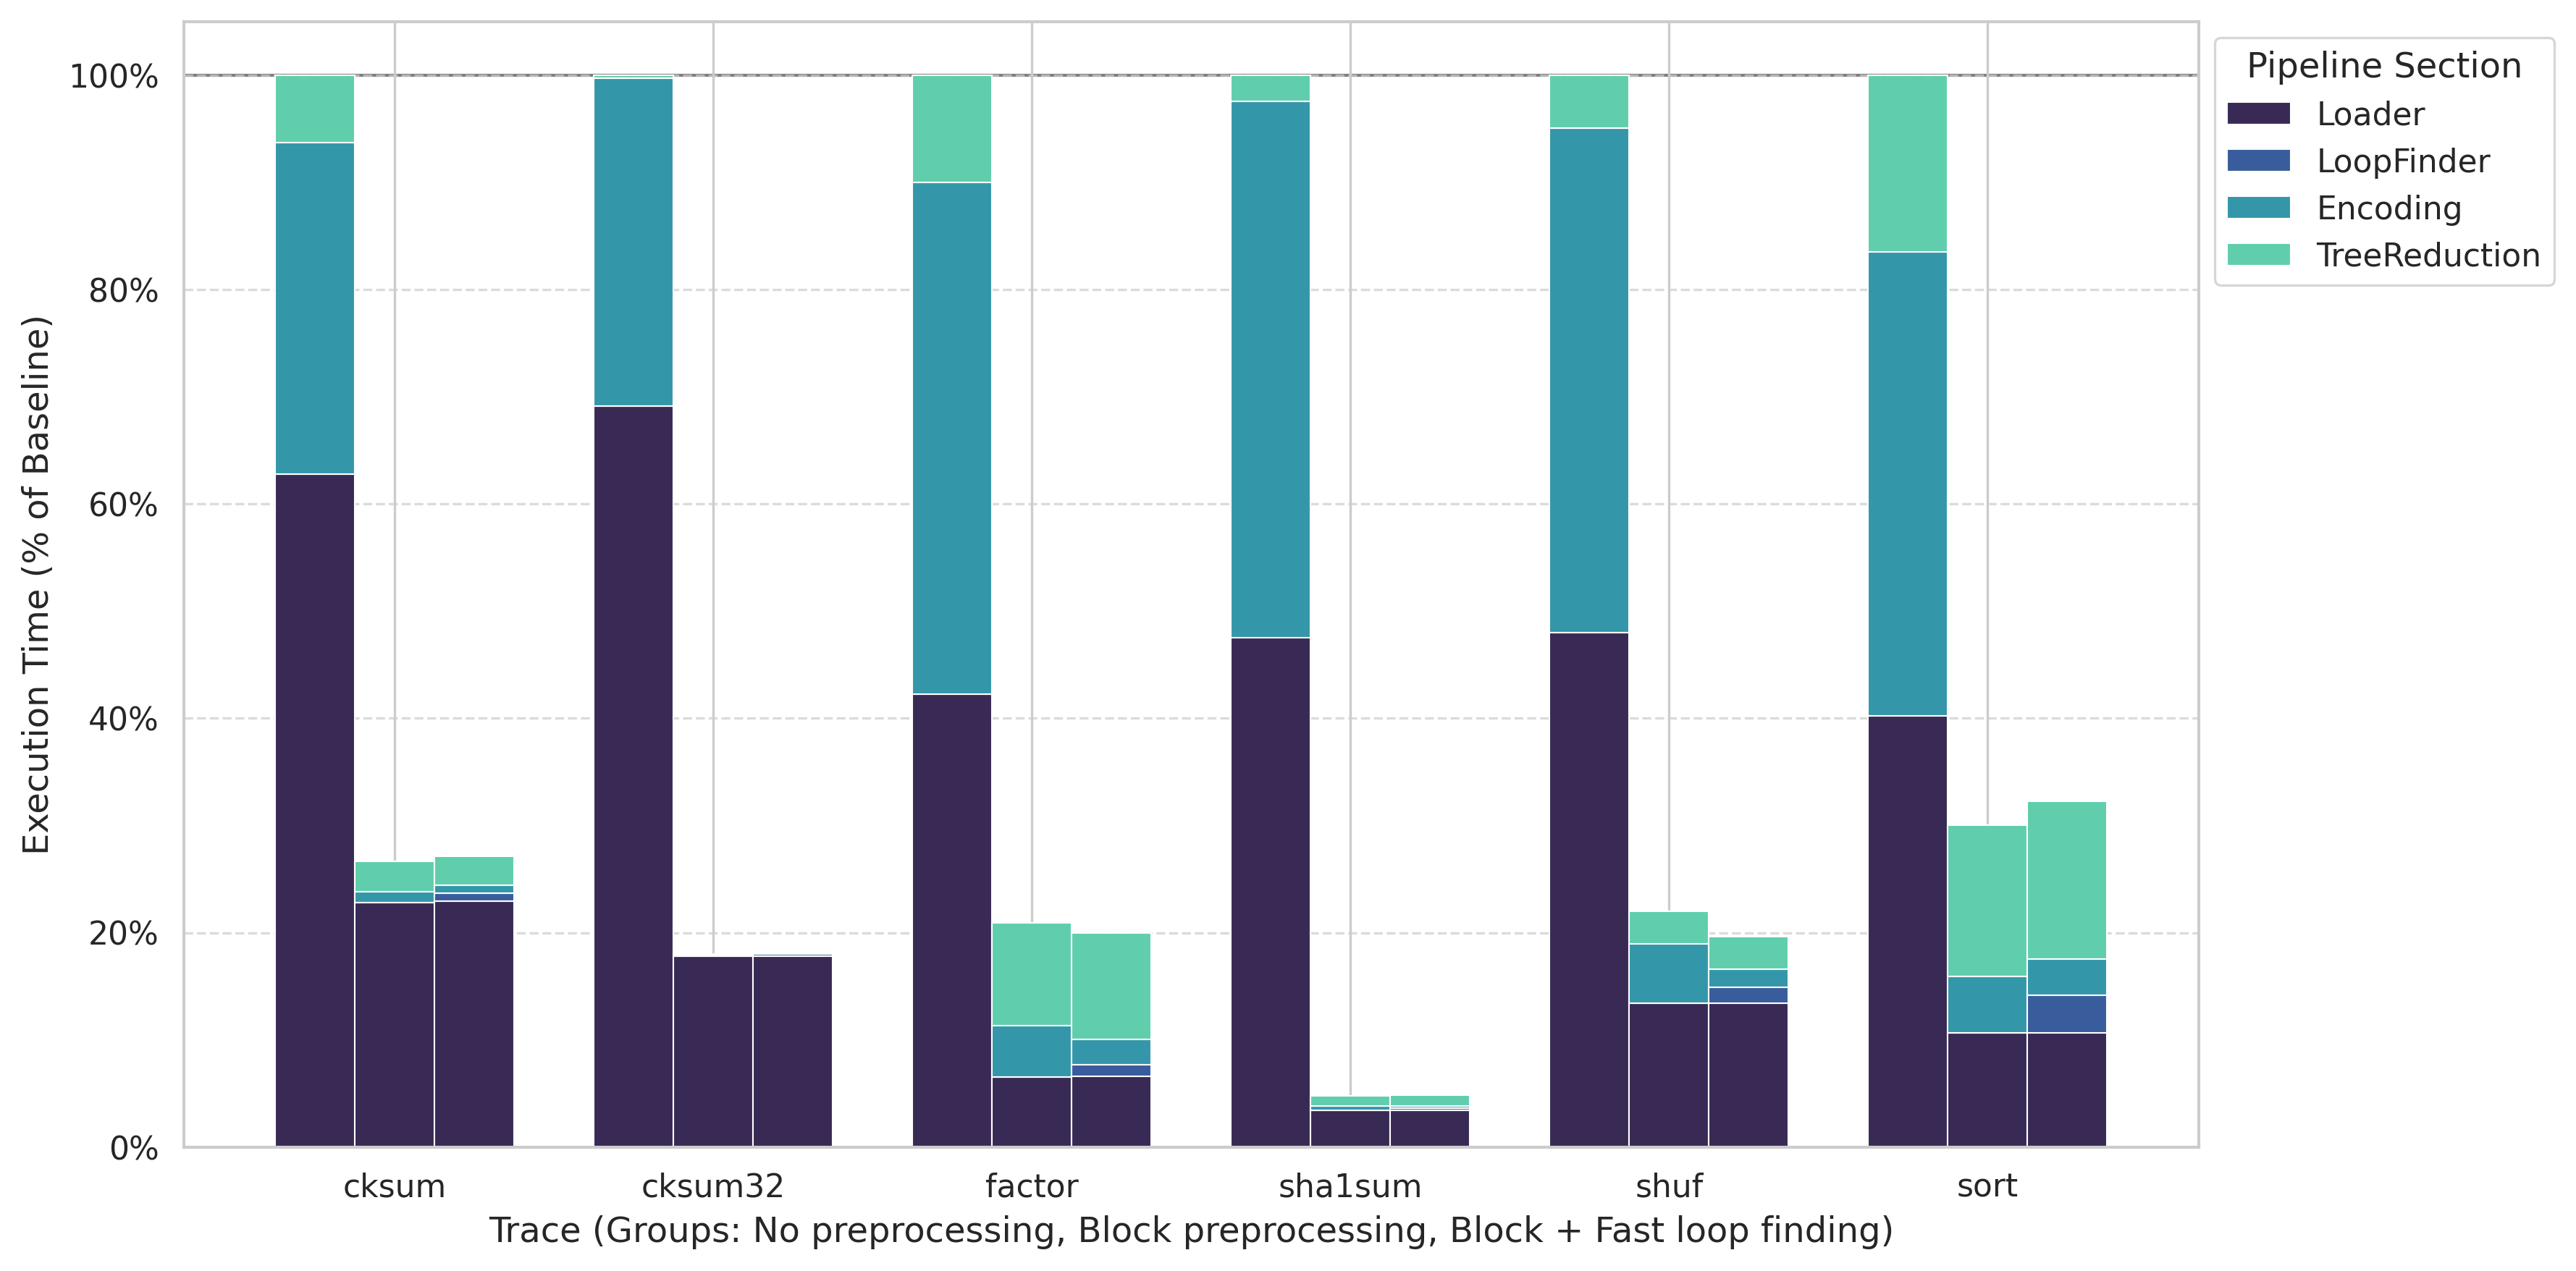
\includegraphics[width=1\textwidth]{graphs/pipeline_optimization.png}
  \caption{Comparing the speedup for block preprocessing and fast loop finding}
  \label{eval:fig:single-thread-speedup}
\end{figure}

\section{Concurrency and GPU deep dive}

encoder time performance (directly from program execution) with threads and chunks

encoder efficiency! with chunk count

multiplication performance (artificial benchmark so we can make sure multiplier doesnt starve for huge multiiplication counts) with threads

GPU timeline

\section{Memory profiling}

bar chart maximum resident set size 

line graph heap memory allocation

\section{Holistic Pipeline}


\chapter{Conclusions}

The project was overall a success. The analysis tool built offers a direct performance improvement over the classical 
techniques for conducting ILP limit studies. All the minimum success criteria were met, and nearly all the extensions have 
been implemented with varying levels of success. The associativity of the matrix approach has been shown to offer 
clear pathways for both data-driven and parallel optimisations.

\section{Lessons learned}



\section{Future work}

While the core of the project is complete, there are further improvements that could be made. Listed are some shortcomings 
that could be addressed in the future.

\begin{itemize}
  \item The GPU pipeline did not make full use of the compute available. More work could be done to optimise the memory 
    layout for contiguous storage, implement a double-buffered dispatch architecture to hide overhead, and make use of
    a hybrid system that simultaneously multiplies matrices on CPU threads to maximise throughput.
  \item The memory usage of the tool is technically unbounded, and it would often crash during benchmarks, or even stall 
    due to spillover into swap space. More work could be done to ensure that the maximum memory usage is safely limited 
    during analysis of realistic traces of trillions of dynamic instructions.
  \item I/O and parsing forms a sequential bottleneck for the analysis tool when loading the initial expression. Work 
    could be done to implement an alternative binary-based format to speed up loading and reduce the bottleneck.
  \item The analysis tool only tracked register dependencies. While this is still useful for smaller subtraces that keep their 
    working set in registers, programs will often spill registers to memory. This happened with all the sample traces,
    and so reported ILP limits were higher than actual values. More work could be done to assess the impact of the data-driven 
    optimisations on the more complex structure of a matrix expression that tracks memory dependencies.
\end{itemize}

Overall, the project achieved its goals, and I think it was an interesting project, bridging gaps between concepts in 
processor design, graph theory, pattern exploitation and parallel computing.


%tc:ignore

%%%%%%%%%%%%%%%%%%%%%%%%%%%%%%%%%%%%%%%%%%%%%%%%%%%%%%%%%%%%%%%%%%%%%
% the bibliography
\cleardoublepage
\phantomsection
\addcontentsline{toc}{chapter}{Bibliography}
\bibliographystyle{plainnat}
\bibliography{references}

%%%%%%%%%%%%%%%%%%%%%%%%%%%%%%%%%%%%%%%%%%%%%%%%%%%%%%%%%%%%%%%%%%%%%
% the appendices
\appendix

\chapter{Mathematical definitions and proofs} \label{apdx:proofs}

\begin{definition}[Semiring] \label{def:semiring}
  A semiring \cite{Wandsnider2020} is a set $R$ along with two operations, addition (+) and multiplication ($\cdot$), which satisfy the 
  following axioms:

  \begin{enumerate}
    \item Addition is associative and commutative.
    \item Multiplication is associative.
    \item There exists an additive identity, which we usually call $\mathbb{0}$. Additionally, $\mathbb{0}$ annihilates 
      $R$, that is, for all $x \in R$, $\mathbb{0} \cdot x = x \cdot \mathbb{0} = \mathbb{0}$.
    \item There exists a multiplicative identity, which we usually call $\mathbb{1}$.
    \item Multiplication left and right distributes over addition.
  \end{enumerate}
\end{definition}

\MatrixExp*
\begin{proof}
  We proceed by induction on $q$, the maximum number of edges in the path.

  \textbf{Base case ($q = 1$):} Consider the matrix $X^1=X$. By the definition of an adjacency matrix, the entry  
  $x_{ij}^{(1)}$ is exactly the weight of the direct edge from node $i$ to node $j$. If no such edge exists, then 
  $x_{ij}^{(1)} = -\infty$. Thus, the base case holds: the entries represent their longest paths consisting of at most 
  one edge.

  \textbf{Inductive step:} Assume the claim holds for $q$. That is the matrix $X^{q}$ has entries $x_{ij}^{q}$ 
  representing the longest path from $i$ to $j$ using at most $q$ edges.
  We show that the claim holds for $q+1$. By definition, $X^{q+1} = X^{q} \odot X$
  The entry $x_{ij}^{(q+1)}$ is calculated as:
  $$x_{ij}^{(q+1)} = \bigoplus{k=1}^{n} (x_{ik}^{(q)}\odot x_{kj})$$
  Translating this to the original operators:
  $$
  x_{ij}^{(q+1)} = \max_{1 \leq k \leq n} (x_{ik}^{(q)} + x_{kj})
  $$
  This lines up perfectly with the dynamic programming approach to finding the longest path. To find a longest path from
  node $i$ to node $j$, it checks every intermediate node $k$. It takes the longest known path from $i$ to $k$ of at most 
  $q$ edges (by the inductive hypothesis), and adds the direct edge cost from $k$ to $j$. By taking the maximum over all 
  intermediate nodes $k$, we find the absolute longest path from $i$ to $j$ of at most $q+1$ edges. Thus the claim holds 
  for all integers $q>0$.
\end{proof}


\chapter{Additional code listings}

\begin{algfloat}[ht]
\begin{lstlisting}[mathescape=true,language=C++]
function multiply(SparseMatrix<m,n> A, SparseMatrix<n,p> B) {
  int[p] x  = [$-\infty$,...,$-\infty$];
  int[p] xb = [-1,...,-1];
  Queue<int>  iCols;
  SparseMatrix<m,p> C;

  IC[0] = 0;

  for (i : [0,...,m-1]) {
    for (jp : [IA[i],...,IA[i+1]-1]) {
      int j = JA[jp];
      int a = VA[jp];

      for (kp : [IB[j],...,IB[j+1]-1]) {
        int k = JB[kp];
        int b = VB[kp];

        if (xb[k] != i) {
          xb[k] = i;
          x[k] = a + b;
          iCols.push(k);
        } else {
          x[k] = max(x[k], a + b);
        }
      }
    }

    while (!iCols.empty) {
      int col = iCols.pop();
      // Assume dynamically allocated arrays
      JC.push(col);
      VC.push(x[col]);
    }

    IC[i+1] = JC.size;
  }

  return C;
}
\end{lstlisting}
\caption{Sparse-Sparse matrix multiplication}
\label{alg:Sp-Sp-matrix}
\end{algfloat}

\begin{algfloat}[htbp]
\begin{lstlisting}[language=C++, caption={Verifying trace ranges match}, label={alg:verify}]
function verifyMatch(int[] trace, int startA, int startB, int length) {
  /* Do a quick boundary check and exit if tails don't match */
  if (startB + length > trace.size()) return false;
  if (trace[startA + length - 1] != trace[startB + length - 1]) return false;

  /* Verify full sequence */
  for (k : [0,...,length-2]) {
    if (trace[startA + k] != trace[startB + k]) {
      return false;
    }
  }
  return true;
}
\end{lstlisting}

\begin{lstlisting}[language=C++, caption={Greedily finding all iterations}, label={alg:iterate}]
function countIterations(int[] trace, int currentPos, int period) {
  int iterations = 2; // Account for original body and first match
  int scanPos = currentPos + period;

  for (scanPos + period <= trace.size()) {
    if (verifyMatch(trace, currentPos, scanPos, period)) {
      iterations++;
      scanPos += period;
    } else {
      break;
    }
  }
  return iterations;
}
\end{lstlisting}
\caption{Helper functions for the fast loop finder. Standard array-scanning logic.}
\label{alg:fast-loop-helper}
\end{algfloat}

\begin{algfloat}[htbp]
\begin{lstlisting}[language=C++, caption={Queueing Logic}, label={alg:queue}]
concurrentMap<Matrix*, MatrixJob> pendingJobs;
concurrentQueue<MatrixJob> readyJobs;

/* Queueing up a new multiplication */
function enqueueMultiplication(MatrixJob newJob) {
  newJob.unresolvedDeps = 2;

  // Safely insert C into the map
  with WriteLock(pendingJobs[newJob.C]) {
    pendingJobs[newJob.C] = newJob;
  }

  checkDependency(A,C);
  checkDependency(B,C);

  // Enqueue if dependencies are resolved.
  with ReadLock(pendingJobs[newJob.C]) {
    if (pendingJobs[newJob.C].unresolvedDeps == 0) {
      readyJobs.push(pendingJobs[newJob.C]);
    }
  }
}
\end{lstlisting}

\begin{lstlisting}[language=C++, caption={Dependency Processing}, label={alg:deps1}]
function checkDependency(Matrix* dependency, Matrix* dependent) {
  with WriteLock(pendingJobs[dependency]) {
    if (dependency in pendingJobs) {
      pendingJobs[dependency].dependents.append(dependent);
    } else {
      // Dependency is complete; update dependent
      with WriteLock(pendingJobs[dependent]) {
        pendingJobs[dependent].unresolvedDeps--;
      }
    }
  }
}
\end{lstlisting}
\caption{Matrix queueing and dependency management logic.}
\label{alg:queue-mults}
\end{algfloat}

\begin{algfloat}[htbp]
    \centering
    \begin{lstlisting}[language=C++, caption={Execution Logic}, label={alg:exec}]
concurrentMap<Matrix*, MatrixJob> pendingJobs;
concurrentQueue<MatrixJob> readyJobs;

void executeMultiplication(MatrixJob job) {
    *(job.C) = *(job.A) * *(job.B);
    processDependents(job.C);
    with WriteLock(pendingJobs[job.C]) {
        pendingJobs.erase(job.C);
    }
}
    \end{lstlisting}

    \vspace{1em} % Adds a small gap between the two listings

    \begin{lstlisting}[language=C++, caption={Dependency Processing}, label={alg:deps2}]
void processDependents(Matrix* dependency) {
    Matrix*[] deps;
    with ReadLock(pendingJobs[dependency]) {
        deps = pendingJobs[dependency].dependents;
    }
    for (Matrix* dep : deps) {
        with WriteLock(pendingJobs[dep]) {
            if (pendingJobs.contains(dep)) {
                pendingJobs[dep].unresolvedDeps--;
                if (pendingJobs[dep].unresolvedDeps == 0) {
                    readyJobs.push(pendingJobs[dep]);
                }
            }
        }
    }
}
    \end{lstlisting}
    \caption{Asynchronous matrix multiplication and dependency management logic.}
    \label{alg:async-mults}
\end{algfloat}

\begin{algfloat}[htbp]
\begin{lstlisting}[language=C++]
#define TILE_SIZE 16
__kernel void batched_max_plus_tiled(__global const int* A_batch,
                                     __global const int* B_batch,
                                     __global int* C_batch,
                                     const int N,
                                     const int negative_infinity) {
  __local int As[TILE_SIZE][TILE_SIZE];
  __local int Bs[TILE_SIZE][TILE_SIZE];

  int bx = get_group_id(0);
  int by = get_group_id(1);
  int tx = get_local_id(0);
  int ty = get_local_id(1);
  int batch_idx = get_group_id(2);

  int row = by * TILE_SIZE + ty;
  int col = bx * TILE_SIZE + tx;
  int offset = batch_idx * (N * N);

  int max_val = negative_infinity;
  int num_tiles = (N + TILE_SIZE - 1) / TILE_SIZE;

  for (int t = 0; t < num_tiles; ++t) {
    if (row < N && (t * TILE_SIZE + tx) < N) {
      As[ty][tx] = A_batch[offset + row * N + t * TILE_SIZE + tx];
    } else {
      As[ty][tx] = negative_infinity;
    }

    if ((t * TILE_SIZE + ty) < N && col < N) {
      Bs[ty][tx] = B_batch[offset + (t * TILE_SIZE + ty) * N + col];
    } else {
      Bs[ty][tx] = negative_infinity;
    }

    barrier(CLK_LOCAL_MEM_FENCE);

    for (int k = 0; k < TILE_SIZE; ++k) {
      int a_val = As[ty][k];
      int b_val = Bs[k][tx];

      if (a_val != negative_infinity && b_val != negative_infinity) {
        int current_path_length = a_val + b_val;
        if (current_path_length > max_val) {
          max_val = current_path_length;
        }
      }
    }
    barrier(CLK_LOCAL_MEM_FENCE);
  }

  if (row < N && col < N) {
    C_batch[offset + row * N + col] = max_val;
  }
}
\end{lstlisting}
  \caption{Tiled GPU kernel for computing batches of matrix multiplications}
  \label{alg:gpu-kernel}
\end{algfloat}

\chapter{Distribution of matrix sparsity in datasets} \label{apdx:nni-histograms}



% \chapter{Analysis tool outputs} \label{apdx:outputs}

\section{Baseline}

cksum:
\lstinputlisting{../tool-outputs/cksum/naive.log}
cksum32:
\lstinputlisting{../tool-outputs/cksum32/naive.log}
factor:
\lstinputlisting{../tool-outputs/factor/naive.log}
sha1sum:
\lstinputlisting{../tool-outputs/sha1sum/naive.log}
shuf:
\lstinputlisting{../tool-outputs/shuf/naive.log}
sort:
\lstinputlisting{../tool-outputs/sort/naive.log}

\section{Matrix-based approach}

cksum:
\lstinputlisting{../tool-outputs/cksum/matrix.log}
cksum32:
\lstinputlisting{../tool-outputs/cksum32/matrix.log}
factor:
\lstinputlisting{../tool-outputs/factor/matrix.log}
sha1sum:
\lstinputlisting{../tool-outputs/sha1sum/matrix.log}
shuf:
\lstinputlisting{../tool-outputs/shuf/matrix.log}
sort:
\lstinputlisting{../tool-outputs/sort/matrix.log}

\chapter{Project Proposal}


\includepdf[pages=-]{../../proposal/proposal.pdf}


% \chapter{A primer of basic \LaTeX \ commands}\label{app:latex-primer}

An example figure looks like the one below in Figure \ref{fig:example-figure}.

\begin{figure}[ht]
    \centering
    \includegraphics[width=0.75\textwidth]{example-image-a}
    \caption{Here's an example figure}
    \label{fig:example-figure}
\end{figure}

For an example footnote, use this syntax\footnote{\href{https://www.cst.cam.ac.uk/}{The CST Department Website}}.

For bullet points:
\begin{itemize}
    \item First item.
    \item Second item.
\end{itemize}

For enumerated lists:
\begin{enumerate}
    \item First item.
    \item Second item.
\end{enumerate}

See Table \ref{tab:example-table} for an example table using the \texttt{booktabs} package. Note the positioning of the caption above the table rather than below for figures.

\begin{table}[h]
\centering
 \caption{The five oldest Cambridge colleges}
 \label{tab:example-table}
    \begin{tabular}{c c c}
        \toprule
         \textbf{\#} & \textbf{College} & \textbf{Founding date} \\
         \midrule
            1 & Peterhouse & 1284 \\
            2 & Clare & 1326 \\
            3 & Pembroke & 1347 \\
            4 & Gonville and Caius & 1348 \\
            5 & Trinity Hall & 1350 \\
         \bottomrule
    \end{tabular}
\end{table}

To cite, we simply use the \texttt{\textbackslash citep\{\}} or \texttt{\textbackslash citet\{\}} command, in combination with a \textit{bibtex} file.

Kitchen supplies are known to go missing in an office context \citep{CaseOfDisappearingTeaspoons}. However, not all hope is lost, nor should we lose faith in humankind's ability to retain teaspoons. For instance, \citet{TeaspoonSolutionProposal} has proposed an elegant solution which could be considered world-changing.

To list code, use the \href{https://www.overleaf.com/learn/latex/Code_listing#Using_listings_to_highlight_code}{\texttt{lstlisting}} package. This contains all kinds of customisation for how code is linted within your \LaTeX \ source files.

\begin{lstlisting}
import java.util.Random;

public class RandomExample {

    public static void main(String[] args) {
        Random random = new Random();

        int[] numbers = new int[5];

        // Fill array with random numbers
        for (int i = 0; i < numbers.length; i++) {
            numbers[i] = random.nextInt(100);
        }

        // Print the numbers
        System.out.println("Generated numbers:");
        for (int num : numbers) {
            System.out.println(num);
        }

        // Simple calculation
        int sum = 0;
        for (int num : numbers) {
            sum += num;
        }

        double average = (double) sum / numbers.length;
        System.out.println("Average: " + average);
    }
}
\end{lstlisting}
%
% \chapter{Formatting Checklist}

\LaTeX documents are easy to format well with little effort. If you're coming from a `what you see is what you get' word processor, use the following (non-exhaustive) checklist to check your report is neatly formatted. Finding out how to use these formatting styles is mainly left as an exercise to the reader.

\begin{itemize}
    \item Are your speech marks correctly formatted?  
    \begin{itemize}
        \item Example: A ``common mistake'' is for users to incorrectly use normal quotation mark characters in their \LaTeX\ files.
        \item Anti-Pattern Example: Some think that computer science is "boring".
    \end{itemize}

    \item Are you using the \href{https://nhigham.com/2019/11/19/better-latex-tables-with-booktabs/}{\texttt{booktabs}} package for neater tables?  

    \item Are you citing correctly?  
    \begin{itemize}
        \item Example: Kitchen supplies are known to go missing in an office context \citep{CaseOfDisappearingTeaspoons}. However,  \citet{TeaspoonSolutionProposal} has proposed an elegant solution.
        \item Anti-Patterns:
        \begin{itemize}
            \item Not putting spaces between text and reference, e.g., Kitchen supplies are known to go missing in an office context\citep{CaseOfDisappearingTeaspoons}.
            \item Incorrect use of \texttt{\textbackslash citep\{\}} or \texttt{\textbackslash citet\{\}}, e.g., Kitchen supplies are known to go missing in an office context \citet{CaseOfDisappearingTeaspoons}. However, \citep{TeaspoonSolutionProposal} has proposed an elegant solution.
        \end{itemize}
    \end{itemize}

    \item Are references to programmatic things (e.g., file, class, or variable names) in a monospaced font?
    \begin{itemize}
        \item Use \texttt{\textbackslash texttt\{\}} for this
    \end{itemize}

    \item Are code extracts formatted as code listings (see Appendix \ref{app:latex-primer})?
    
    \item Is the text in your figures readable?  

    \item Are all of your paragraphs evenly spaced?  

    \item Are you using math mode when using equations/symbols?  

    \item Are your captions for figures appearing below figures and captions for tables appearing above them?
    \begin{itemize}
        \item Anti-Patterns:
        \begin{itemize}
            \item Putting captions in wrong place.
            \item Not including captions at all.
        \end{itemize}
    \end{itemize}

    \item Are your titles, section headings, and captions in sentence case?
    \begin{itemize}
        \item Example: \textbf{My new type system for Rust}
        \item Anti-pattern: \textbf{My New Type System For Rust}
    \end{itemize}

    \item Are your footnotes appearing immediately after a word?
    \begin{itemize}
        \item Example: This program was written in Python\footnote{Version 3.12 at the time of writing}.
        \item Anti-Pattern: This experiment was conducted in January 2025 \footnote{Apart from one participant, who took part in April 2025.}.
    \end{itemize}

    \item Are there sufficient details in your references?
    \begin{itemize}
        \item Example: See the detail of references included in \citet{CaseOfDisappearingTeaspoons}.
        \item Anti-Pattern: Missing key information such as the year published, all of the authors of the work, the DOI if applicable, etc. See \citet{BadReference} for an example of a poor reference.
    \end{itemize}

\end{itemize}

%%%%%%%%%%%%%%%%%%%%%%%%%%%%%%%%%%%%%%%%%%%%%%%%%%%%%%%%%%%%%%%%%%%%%%%%%%%%%%%%
%% Index:
%%
%\printthesisindex

%tc:endignore
\end{document}
